

\documentclass[a4paper,8pt]{extarticle} % extarticle allows to use font size of 8pt.

\usepackage[a4paper, top=1.6cm, bottom=2cm, left=1.6cm, right=1.6cm]{geometry} % Marge reduction.

%% Language specific package
\usepackage[french]{babel}
\frenchbsetup{StandardLists=true} % Necessary to use enumitem with babel/french.

%% Font and typing packages
\usepackage{fontspec}
\setmainfont[
	Ligatures=TeX,
	ItalicFont={Dancing Script},
	BoldItalicFont={Dancing Script}
	]{PT Serif} % default is Latin Modern
\newfontfamily\antiquefont[Ligatures=TeX]{Caslon Antique} % fancy font
\usepackage{microtype}			% Greatly improves general appearance of the text.
\usepackage{SIunits}			% Unit appearance.
\usepackage{xspace}				% Define commands that appear not to eat spaces.
\usepackage{ulem}				% To cross words out. Use \sout{}.

%% Array utilities
\usepackage{array}				% Additionnal options for arrays.
\usepackage{colortbl}			% Additionnal options for coloring arrays.
\usepackage[table]{xcolor}		% Auto alternate grey-white rows.
\usepackage[export]{adjustbox}		% Centered pics in tables

%% List utilities
\usepackage[inline]{enumitem}   % Display inline lists.
\usepackage{etoolbox}           % General utility. Good for lists for instance.
\usepackage{xparse}             % List utilities.
\usepackage{datatool}	% Handling alphabetical order.

%% Frames
\usepackage{framed}				% Boxes.
\usepackage[framemethod=TikZ]{mdframed}% For fancy frames.
\usepackage{tikz}				% For fancy frames.
\usepackage{wrapfig}			% Fancy insertion of pics in text.

%% Page utilities
\usepackage{multicol}			% Allows to divide a part of the page in multiple columns.
	
%% Others
\usepackage{keyval}             % Used to create maps of commands/labels/objects.
	\makeatletter                  % Mandatory for the usage of keyval.
\usepackage{xstring}            % String parsing, cutting, etc.
\usepackage{hyperref} % Links in PDF.


%%% Update of the dotfill command to always get dots

\newcommand{\predotfill}{\penalty0\hbox{}\nobreak}%


%%% Command to avoid typing \xspace when creating a new name macro

\newcommand{\newnamemacro}[2]{\newcommand{#1}{#2}} % \xspace removed for compatibility with alphabetical ordering

%%% Language specific stuff


\newcommand{\translationteam}{\item \og AEnoriel \fg \item \og Anglachel \fg \item \og Astadriel \fg \item \og Batcat \fg \item \og Bigfish \fg \item \og Eru \fg  \item \og Gandarin \fg \item \og Groumbahk \fg \item \og Iluvatar \fg \item \og Mammstein \fg \item \og Shlagrabak \fg \item et beaucoup d'autres...}

\hypersetup{
	pdfauthor={Équipe de traduction française de T9A},
	pdfsubject={Règles pour le jeu Batailles Fantastiques : Le 9\ieme{} Âge},
}

%%% Commands %%%

\ifdef{\isitanAB}{

\newcommand{\addtosortedlist}[1]{%
	\protected@edef\textarg{#1}%
	\protected@edef\textwithoutspaces{\expandafter\removespaces\expandafter{\textarg}}%
	\substitute\textwithoutspaces{É}{E}% Most used special characters of the language, and equivalent for alphabetical ordering
	\substitute\textwithoutspaces{È}{E}%
	\substitute\textwithoutspaces{Ê}{E}%
	\substitute\textwithoutspaces{é}{e}%
	\substitute\textwithoutspaces{è}{e}%
	\substitute\textwithoutspaces{ê}{e}%
	\substitute\textwithoutspaces{À}{A}%
	\substitute\textwithoutspaces{à}{a}%
	\substitute\textwithoutspaces{ù}{u}%
	\expandafter\sortitem\expandafter[\textwithoutspaces]{#1}%
}%

\newcommand{\pts}[1]{% First step is to remove spaces if there are some
	\def\numberwithoutspaces{\expandafter\removespaces\expandafter{#1}}%
	% Next step is getting rid of formatting if there are any (bold, color, ...)
	\pdfstringdef\cleannumber{\numberwithoutspaces}%
	% Now we can try if it is 1 or not
	\expandafter\ifstrequal\expandafter{\cleannumber}{1}{#1~\labels@point}{%
	\expandafter\ifstrequal\expandafter{\cleannumber}{0.5}{0,5~\labels@point}{%
	\expandafter\ifstrequal\expandafter{\cleannumber}{1.5}{1,5~\labels@point}{%
	#1~\labels@points}}}%
}

}{}

% Dark gods
\newcommand{\dchange}{Changement}
\newcommand{\dlust}{Luxure}
\newcommand{\pestilence}{Pestilence}
\newcommand{\wrath}{Courroux}
\newcommand{\truechaos}{Chaos Primordial}


% Nothing to edit here

\ifdef{\isitanAB}{

\newcommand{\alliancepts}[1]{
\ifsubstring{#1}{\free}{%
		\free{}%
	}{%
	\ifsubstring{#1}{\permodel}{%
		\splitatinf{#1}\myoption\myvalue%
		\pts{\myvalue}\permodel{}%
	}{%
	\pts{#1}
	}}
}

% You might wanna change the order of the gods - advanced user
\newcommand{\allianceoptions}[1]{%
	\defallianceoptions{#1}%
	\unitentryformat{\labels@allianceoptions\spacebeforecolon{}:}\newline
	\expandafter\ifblank\expandafter{\allianceoptions@introsentence}{}{\noindent\allianceoptions@introsentence{}\spacebeforecolon{}:}
	
	\expandafter\ifblank\expandafter{\allianceoptions@wrath}{
		\setlength{\columnseprule}{0.5pt}
		\renewcommand{\columnseprulecolor}{\color{black!30}}
		\vspace*{-0.2cm}\begin{multicols}{3}\raggedcolumns
		
			\begin{center}
			\noindent\dchange{}
			
			\noindent\alliancepts{\allianceoptions@change}
			\vspace*{-0.3cm}
			\end{center}
		
		\columnbreak
		
			\begin{center}
			\noindent\dlust{}
			
			\noindent\alliancepts{\allianceoptions@lust}
			\vspace*{-0.3cm}
			\end{center}
		
		\columnbreak

			\begin{center}
			\noindent\pestilence{}
			
			\noindent\alliancepts{\allianceoptions@pestilence}
			\vspace*{-0.3cm}
			\end{center}
			
		\end{multicols}
		\setlength{\columnseprule}{0pt}	
	}{
		\setlength{\columnseprule}{0.5pt}
		\renewcommand{\columnseprulecolor}{\color{black!30}}
		\vspace*{-0.2cm}\begin{multicols}{4}\raggedcolumns
		
			\begin{center}
			\noindent\dchange{}
			
			\noindent\alliancepts{\allianceoptions@change}
			\vspace*{-0.3cm}
			\end{center}
		
		\columnbreak

			\begin{center}
			\noindent\wrath{}
			
			\noindent\alliancepts{\allianceoptions@wrath}
			\vspace*{-0.3cm}
			\end{center}
		
		\columnbreak
		
			\begin{center}
			\noindent\dlust{}
			
			\noindent\alliancepts{\allianceoptions@lust}
			\vspace*{-0.3cm}
			\end{center}
		
		\columnbreak

			\begin{center}
			\noindent\pestilence{}
			
			\noindent\alliancepts{\allianceoptions@pestilence}
			\vspace*{-0.3cm}
			\end{center}
			
		\end{multicols}
		\setlength{\columnseprule}{0pt}
	}
}

}{}


%%% Labels %%%

% Profile

\newcommand{\labels@M}{M}
\newcommand{\labels@WS}{CC}
\newcommand{\labels@BS}{CT}
\newcommand{\labels@S}{F}
\newcommand{\labels@T}{E}
\newcommand{\labels@W}{PV}
\newcommand{\labels@I}{I}
\newcommand{\labels@A}{A}
\newcommand{\labels@Ld}{Cd}
\newcommand{\labels@Invocation}{Invocation} % For Vampire Covenant profiles
\newcommand{\labels@roundbase}{rond} % printed after XX mm for round bases

\newcommand{\Strength}{Force}

% Technical

\newcommand{\labels@range}{Portée}
\newcommand{\labels@point}{pt}
\newcommand{\labels@points}{pts}
\newcommand{\labels@only}{uniquement}
\newcommand{\labels@magic}{Magie}
\newcommand{\labels@pathsused}{Génère ses sorts dans la Discipline}
\newcommand{\labels@model}{figurine}
\newcommand{\labels@models}{figurines}
\newcommand{\labels@Singlemodel}{Figurine \textbf{seule}}

% Unit entry labels

\newcommand{\labels@basesize}{Socle}
\newcommand{\labels@trooptype}{Type de troupe}
\newcommand{\labels@specialrules}{Règles Spéciales}
\newcommand{\labels@alignment}{Allégeance}
\newcommand{\labels@alliance}{Allégeance}
\newcommand{\labels@allianceoptions}{Options d'Allégeance}
\newcommand{\labels@greenhiderace}{Race de Peaux Vertes}
\newcommand{\labels@equipment}{Équipement}
\newcommand{\labels@weapons}{Armes}
\newcommand{\labels@armour}{Armure}
\newcommand{\labels@options}{Options}
\newcommand{\labels@commandgroup}{État-Major}
\newcommand{\labels@charactermounts}{Montures de Personnages}
\newcommand{\labels@mounts}{Montures}
\newcommand{\labels@mount}{Monture}
\newcommand{\labels@specialequipment}{Équipement Spécial}

% Command groups

\newcommand{\labels@champion}{Champion}
\newcommand{\labels@standardbearer}{Porte-Étendard}
\newcommand{\labels@musician}{Musicien}
\newcommand{\labels@singlebannerallowance}{Une seule unité de ce type peut prendre une Bannière Magique}
\newcommand{\labels@condsinglebannerallowance}{Une seule unité de ce type peut prendre une Bannière Magique si}
\newcommand{\labels@bannerallowance}{Bannière Magique}
\newcommand{\labels@veteranstandardbearer}{Peut devenir Porte-Étendard Vétéran}
\newcommand{\labels@championallowance}{Arme Magique}

% Titles

\newcommand{\labels@armylist}{Liste des Troupes}
\newcommand{\labels@lords}{Seigneurs}
\newcommand{\labels@heroes}{Héros}
\newcommand{\labels@coreunits}{Unités de Base}
\newcommand{\labels@specialunits}{Unités Spéciales}
\newcommand{\labels@rareunits}{Unités Rares}
\newcommand{\labels@armywiderules}{Règles Communes de l'Armée}
\newcommand{\labels@armyspecialrules}{Règles Spéciales de l'Armée}
\newcommand{\labels@armoury}{Armurerie}
\newcommand{\labels@magicalitems}{Objets Magiques}
\newcommand{\labels@magicalweapons}{Armes Magiques}
\newcommand{\labels@magicalarmour}{Armures Magiques}
\newcommand{\labels@talismans}{Talismans}
\newcommand{\labels@enchanteditems}{Objets Enchantés}
\newcommand{\labels@arcaneitems}{Objets Cabalistiques}
\newcommand{\labels@magicalbanners}{Bannières Magiques}
\newcommand{\labels@quickrefsheet}{Fiche de Référence}
\newcommand{\labels@changelog}{Change Log}

\newcommand{\labels@lordsInitial}{S}
\newcommand{\labels@heroesInitial}{H}
\newcommand{\labels@coreunitsInitial}{B}
\newcommand{\labels@specialunitsInitial}{S}
\newcommand{\labels@rareunitsInitial}{R}
\newcommand{\labels@mountsInitial}{M}


% Titlepage

\newcommand{\labels@fantasybattles}{Batailles Fantastiques}
\newcommand{\labels@NinthAge}{Le 9\ieme{} Âge}
\newcommand{\labels@armyrules}{Règles de l'Armée}
\newcommand{\labels@frontpagecredits}{%
\labels@fantasybattles{} : \labels@NinthAge{} est un jeu créé et entretenu par la communauté qui met en scène des affrontements de figurines.\newline
Toutes les règles sont disponibles gratuitement sur le site suivant. Vos retours et suggestions sont les bienvenus : \url{http://www.the-ninth-age.com/}
}
\newcommand{\labels@license}{Copyright Creative Commons license : \url{the-ninth-age.com/license.html}}
\newcommand{\labels@tableofcontents}{Sommaire}
\newcommand{\labels@introduction}{%
\begin{center}\noindent{\Largerfontsize\textbf{Note des traducteurs}}\end{center}
\vspace{0.5cm}

Nous souhaitons remercier chaleureusement l'équipe à l'initiative du 9\ieme{} Âge pour leur motivation et leur travail continu pour faire vivre notre passion. Nous espérons que ce jeu saura développer les qualités pour plaire au plus grand nombre et réunir les joueurs, amateurs comme habitués des tournois, autour de règles amusantes et équilibrées, pour finalement s'imposer comme un standard du jeu de figurines. Une grande ambition qui ne pourra s'accomplir que \textbf{grâce à vous}, la communauté, via des retours constructifs, afin de modeler le jeu selon nos désirs. N'étant \textbf{en aucun cas à but lucratif}, le 9\ieme{} Âge part avec un avantage considérable. Les règles des éventuelles nouvelles sorties ne sont pas dictées par le besoin de vendre ces nouveautés. Vous pouvez choisir et acheter vos figurines où bon vous semble, il n'y a pas un unique revendeur toléré. Enfin, vous pouvez être assurés que tant que le 9\ieme{} Âge sera joué, vous disposerez d'un \textbf{support continu et régulier}, celui-ci étant offert par la communauté.

Concernant la traduction en elle-même, nous avons fait de notre mieux pour vous offrir une version de qualité, dont nous espérons qu'elle surpasse celle de la version originale ! Si vous constatez des coquilles, des erreurs, merci de nous les signaler en nous contactant sur le forum du 9\ieme{} Âge, dans le \textbf{sous-forum français} (\url{http://www.the-ninth-age.com/index.php?board/117-french/}). Vous y trouverez aussi les dernières mises à jour. \textbf{En cas de conflit d'interprétation avec la version originale, la version originale fait référence}.

\vspace{0.5cm}
Que ce jeu vous apporte d'innombrables heures de plaisir partagé !

\vspace{1cm}

\ifdef{\translationteam}{
	\begin{multicols}{3}
	\begin{itemize}
		\translationteam
	\end{itemize}
	\end{multicols}
}{}
}
\newcommand{\labels@rulechanges}{% blank ATM
}
\newcommand{\labels@latexcredit}{Document réalisé à l'aide de \LaTeX .}


%%% Technical commands

\newcommand{\only}[1]{(#1 uniquement)}
\newcommand{\free}{gratuit}
\newcommand{\upto}{jusqu'à}
\newcommand{\Upto}{Jusqu'à}
\newcommand{\unlimited}{pas de limite}
\newcommand{\permodel}{/fig.}
\newcommand{\listlastchoice}{ ou}
\newcommand{\notif}[1]{(pas #1)}
\newcommand{\wordand}{et}
\newcommand{\wordwith}{avec}
\newcommand{\ifNmodelsorless}[1]{(#1 figurines ou moins)}
\newcommand{\unitwith}{unité avec}
\newcommand{\From}{De} % From ... to ... models
\newcommand{\wordto}{à}
\newcommand{\wordAll}{Tous}
\newcommand{\spacebeforecolon}{ } % French put a space before colons
\newcommand{\minprice}{Coût min. :}
\newcommand{\mincostfor}{Coût min. pour}
\newcommand{\maxunitsize}{Taille max.}
\newcommand{\additionalfigscost}{Les figurines additionnelles coûtent}


%%% Special rules %%%

\newcommand{\ambush}{Embuscade}
\newcommand{\armourpiercing}[1]{Perforant\ifblank{#1}{}{ (#1)}}
\newcommand{\bodyguard}[1]{Garde du Corps\ifblank{#1}{}{ (#1)}}
\newcommand{\breathweapon}[1]{Attaque de Souffle\ifblank{#1}{}{ (#1)}}
\newcommand{\channel}{Canalisation}
\newcommand{\crushattack}{Attaque Écrasante}
\newcommand{\daemonicinstability}{Instabilité Démoniaque}
\newcommand{\devastatingcharge}{Charge Dévastatrice}
\newcommand{\distracting}{Distrayant}
\newcommand{\divineattacks}{Attaques Divines}
\newcommand{\engineer}{Ingénieur}
\newcommand{\ethereal}{Éthéré}
\newcommand{\fastcavalry}{Cavalerie Légère}
\newcommand{\fear}{Peur}
\newcommand{\fightinextrarank}{Combat avec un Rang Supplémentaire}
\newcommand{\fireborn}{Né du Feu}
\newcommand{\flamingattacks}{Attaques Enflammées}
\newcommand{\flammable}{Inflammable}
\newcommand{\frenzy}{Frénésie}
\newcommand{\fly}[1]{Vol\ifblank{#1}{}{ (#1)}}
\newcommand{\grindingattacks}[1]{Attaques de Broyage\ifblank{#1}{}{ (#1)}}
\newcommand{\hardtarget}{Camouflé}
\newcommand{\hatred}{Haine}
\newcommand{\hellfire}{Feu Démoniaque}
\newcommand{\hidden}{Caché}
\newcommand{\holyattacks}{Attaques Divines} % deprecated, still has to be filled. same as Divine Attacks.
\newcommand{\immunetopsychology}{Immunisé à la Psychologie}
\newcommand{\impacthits}[1]{Touches d'Impact\ifblank{#1}{}{ (#1)}}
\newcommand{\insignificant}{Insignifiant}
\newcommand{\largetarget}{Grande Cible}
\newcommand{\lethalstrike}{Coup Fatal}
\newcommand{\lightningattacks}{Attaques Foudroyantes}
\newcommand{\lightningreflexes}{Réflexes Foudroyants}
\newcommand{\lighttroops}{Troupe Légère}
\newcommand{\magicresistance}[1]{Résistance à la Magie\ifblank{#1}{}{ (#1)}}
\newcommand{\magicalattacks}{Attaques Magiques}
\newcommand{\metalshifting}{Fusion du Métal}
\newcommand{\moveorfire}{Mouvement ou Tir}
\newcommand{\multipleshots}[1]{Tirs Multiples\ifblank{#1}{}{ (#1)}}
\newcommand{\multiplewounds}[2]{Blessures Multiples\ifblank{#1}{}{ (#1\ifblank{#2}{)}{, #2)}}}
\newcommand{\notaleader}{Pas un Meneur}
\newcommand{\otherworldly}{D'Outre-Monde}
\newcommand{\pathmaster}[1]{Maître de la Voie\ifblank{#1}{}{ (#1)}}
\newcommand{\poisonedattacks}{Attaques Empoisonnées}
\newcommand{\quicktofire}{Tir Rapide}
\newcommand{\randommovement}[1]{Mouvement Aléatoire\ifblank{#1}{}{ (#1)}}
\newcommand{\randomattacks}[1]{Attaques Aléatoires\ifblank{#1}{}{ (#1)}}
\newcommand{\regeneration}[1]{Régénération\ifblank{#1}{}{ (#1+)}}
\newcommand{\reload}{Rechargez !}
\newcommand{\requirestwohands}{Arme à deux Mains}
\newcommand{\scythes}{Faux}
\newcommand{\scout}{Éclaireur}
\newcommand{\scouts}{Éclaireurs}
\newcommand{\stomp}[1]{Piétinement\ifblank{#1}{}{ (#1)}}
\newcommand{\strider}[1]{Guide\ifblank{#1}{}{ (#1)}}
\newcommand{\stubborn}{Tenace}
\newcommand{\stupidity}{Stupidité}
\newcommand{\skirmisher}{Tirailleur}
\newcommand{\skirmishers}{Tirailleurs}
\newcommand{\sweepingattack}{Attaque au Passage}
\newcommand{\swiftstride}{Course Rapide}
\newcommand{\thunderouscharge}{Charge Tonitruante}
\newcommand{\terror}{Terreur}
\newcommand{\toxicattacks}{Attaques Toxiques}
\newcommand{\unbreakable}{Indémoralisable}
\newcommand{\undead}{Mort-Vivant}
\newcommand{\unstable}{Instable}
\newcommand{\unwieldy}{Encombrant}
\newcommand{\vanguard}{Avant-Garde}
\newcommand{\volleyfire}{Tir de Volée}
\newcommand{\warplatform}{Plateforme de Guerre}
\newcommand{\wardsave}[1]{Sauvegarde Invulnérable\ifblank{#1}{}{ (#1+)}}
\newcommand{\weaponmaster}{Maître d'Ar\-mes}
\newcommand{\wizardconclave}[1]{Conclave de Sorciers\ifblank{#1}{}{ (#1)}}


%%% Magic %%%


% General

\newcommand{\Pathof}{Voie}

\newcommand{\battle}{Commune}

\newcommand{\anyofthebattlemagic}{dans n'importe laquelle des Voies Communes}
\newcommand{\ONLYanyofthebattlemagic}{Commune de votre choix}

\newcommand{\magiclevel}[1]{\ifnumcomp{#1}{<}{3}{Apprenti Magicien}{Maître Magicien} Niveau #1}
\newcommand{\Level}{Niveau}

\newcommand{\wizard}{Magicien}
\newcommand{\wizards}{Magiciens}

\newcommand{\learnedspell}{Sort Appris}
\newcommand{\learnedspells}{Sorts Appris}
\newcommand{\attributespell}{Attribut de la Voie}
\newcommand{\attributespells}{Attributs de la Voie}
\newcommand{\attributespellnumber}{A}
\newcommand{\traitspell}{Sort Caractéristique}
\newcommand{\traitspells}{Sorts Caractéristiques}
\newcommand{\traitspellnumber}{C}


\newcommand{\boundspell}[1]{Objet de Sort\ifblank{#1}{}{, Puissance #1}}
\newcommand{\boundspells}[1]{Objets de Sort\ifblank{#1}{}{, Puissance #1}}

% Casting Vocabulary

\newcommand{\lostfocus}{Perte de Concentration}
\newcommand{\miscast}{Fiasco}
\newcommand{\miscasts}{Fiascos}
\newcommand{\overwhelmingpower}{Pouvoir Irrésistible}

\newcommand{\breachintheveil}{Brèche dans le Voile}
\newcommand{\catastrophicdetonation}{Explosion Catastrophique}
\newcommand{\witchfire}{Feu de Sorcières}
\newcommand{\sorcerousbacklash}{Contrecoup Magique}
\newcommand{\amnesia}{Amnésie}

% Spell Types

\newcommand{\augment}{Amélioration}
\newcommand{\hex}{Malédiction}
\newcommand{\universal}{Universel}
\newcommand{\missile}{Projectile}
\newcommand{\damage}{Dégâts}
\newcommand{\direct}{Direct}
\newcommand{\focused}{Focalisé}
\newcommand{\vortex}{Vortex}
\newcommand{\ground}{Marqueur}
\newcommand{\linetemplate}{Gabarit de Ligne}
\newcommand{\specialTYPE}{Spécial}
\newcommand{\aura}{Aura}
\newcommand{\castersunit}{Unité du Lanceur}
\newcommand{\caster}{Lanceur}

\newcommand{\template}{Gabarit}

% Spell Durations

\newcommand{\lastsoneturn}{Dure un Tour}
\newcommand{\instant}{Immédiat}
\newcommand{\permanent}{Permanent}
\newcommand{\remainsinplay}{Reste en Jeu}


% Battle Magic

\newcommand{\alchemy}{de l'Alchimie}
\newcommand{\alchemyattribute}{Édit de Fer}
\newcommand{\alchemysignature}{Métal Fondu}
\newcommand{\alchemyspellone}{Lames Enchantées}
\newcommand{\alchemyspelltwo}{Corrosion Rampante}
\newcommand{\alchemyspellthree}{Manteau de Vif-Argent}
\newcommand{\alchemyspellfour}{Pieu d'Argent}
\newcommand{\alchemyspellfive}{Fléau de l'Acier}
\newcommand{\alchemyspellsix}{Transmutation en Or}

\newcommand{\death}{de la Mort}
\newcommand{\deathattribute}{Nuage de Désespoir}
\newcommand{\deathsignature}{Le Baiser de la Faucheuse}
\newcommand{\deathspellone}{Malédiction du Mortel}
\newcommand{\deathspelltwo}{Esprits Dévorants}
\newcommand{\deathspellthree}{Sangsue Psychique}
\newcommand{\deathspellfour}{Moisson d’Âmes}
\newcommand{\deathspellfive}{L’Abîme aussi te Regarde...}
\newcommand{\deathspellsix}{Maelström d’Âmes}

\newcommand{\fire}{du Feu}
\newcommand{\fireattribute}{Feu Déchaîné}
\newcommand{\firesignature}{Boule de Feu}
\newcommand{\firespellone}{Cascade Ardente}
\newcommand{\firespelltwo}{Épées Flamboyantes}
\newcommand{\firespellthree}{Jet de Flammes}
\newcommand{\firespellfour}{Traits Enflammés}
\newcommand{\firespellfive}{Remparts Incandescents}
\newcommand{\firespellsix}{Souffler sur les Braises}

\newcommand{\heavens}{des Cieux}
\newcommand{\heavensattribute}{Second Sceau}
\newcommand{\heavenssignature}{Aquilon}
\newcommand{\heavensspellone}{Bourrasque}
\newcommand{\heavensspelltwo}{Choc Foudroyant}
\newcommand{\heavensspellthree}{Conjonction Astrale}
\newcommand{\heavensspellfour}{Fléau du Ponant}
\newcommand{\heavensspellfive}{Déluge d'Éclairs}
\newcommand{\heavensspellsix}{Appel de la Comète}

\newcommand{\light}{de la Lumière}
\newcommand{\lightattribute}{Lumière Gardienne}
\newcommand{\lightsignature}{Éclat Brûlant}
\newcommand{\lightspellone}{Bouclier Protecteur}
\newcommand{\lightspelltwo}{Étincelle de Courage}
\newcommand{\lightspellthree}{Vitesse Fulgurante}
\newcommand{\lightspellfour}{Toile Scintillante}
\newcommand{\lightspellfive}{Distorsion Temporelle}
\newcommand{\lightspellsix}{Bannissement Divin}

\newcommand{\nature}{de la Nature}
\newcommand{\natureattribute}{Souffle de Vie}
\newcommand{\naturesignature}{Eaux Vivifiantes}
\newcommand{\naturespellone}{Maître de la Terre}
\newcommand{\naturespelltwo}{Le Trône de Chêne}
\newcommand{\naturespellthree}{Esprits des Bois}
\newcommand{\naturespellfour}{Croissance Estivale}
\newcommand{\naturespellfive}{Peau Rocailleuse}
\newcommand{\naturespellsix}{Créatures Souterraines}

\newcommand{\shadows}{des Ombres}
\newcommand{\shadowsattribute}{Course Parmi les Ombres}
\newcommand{\shadowssignature}{Miasmes Obscurs}
\newcommand{\shadowsspellone}{Orbe de Noirceur}
\newcommand{\shadowsspelltwo}{Partir en Fumée}
\newcommand{\shadowsspellthree}{Expérience de Mort Imminente}
\newcommand{\shadowsspellfour}{Char Vaporeux}
\newcommand{\shadowsspellfive}{Ombres Dévorantes}
\newcommand{\shadowsspellsix}{Scalpel Psychique}

\newcommand{\wilderness}{de la Sauvagerie}
\newcommand{\wildernessattribute}{La Chasse Sauvage}
\newcommand{\wildernesssignature}{La Bête qui Sommeille}
\newcommand{\wildernessspellone}{Essaim d’Insectes}
\newcommand{\wildernessspelltwo}{Rage Intérieure}
\newcommand{\wildernessspellthree}{Pieu de Rougebois}
\newcommand{\wildernessspellfour}{Calamité des Bois Sauvages}
\newcommand{\wildernessspellfive}{Tempête Furieuse}
\newcommand{\wildernessspellsix}{Métamorphose
Monstrueuse}

\newcommand{\eightpaths}{Octuple}



% Army Specific Magic

\newcommand{\butchery}{de la Boucherie}
\newcommand{\butcheryattribute}{Sang de Kholag}
\newcommand{\butcherysignature}{Briseur de Dents}
\newcommand{\butcheryspellone}{Buveur de Moelle}
\newcommand{\butcheryspelltwo}{Festin de Tripaille}
\newcommand{\butcheryspellthree}{Concasseur d’Os}
\newcommand{\butcheryspellfour}{Gobeur de Cervelle}
\newcommand{\butcheryspellfive}{Cœur de Troll}
\newcommand{\butcheryspellsix}{Gosier de Géant}

\newcommand{\change}{du Changement}
\newcommand{\changeattribute}{Vent du Changement}
\newcommand{\changesignature}{Feu Azur}
\newcommand{\changespellone}{Feu Rose}
\newcommand{\changespelltwo}{Vague du Changement}
\newcommand{\changespellthree}{Secrets Volés}
\newcommand{\changespellfour}{Règne de la Confusion}
\newcommand{\changespellfive}{Inéluctable Trahison}
\newcommand{\changespellsix}{Portail Éternel}

\newcommand{\thebiggreengods}{des Grands Dieux Verts}
\newcommand{\thebiggreengodsattribute}{Chopez-les !}
\newcommand{\thebiggreengodssignature}{L'Heure de la Raclée}
\newcommand{\thebiggreengodsspellone}{Coup de Boule}
\newcommand{\thebiggreengodsspelltwo}{Poings Bastonneurs}
\newcommand{\thebiggreengodsspellthree}{Même Pas Mal !}
\newcommand{\thebiggreengodsspellfour}{Grande Main Verte}
\newcommand{\thebiggreengodsspellfive}{Boum !}
\newcommand{\thebiggreengodsspellsix}{Le Gros Piétinement}

\newcommand{\thelittlegreengods}{des Petits Dieux Verts}
\newcommand{\thelittlegreengodsattribute}{Fourbe Larcin}
\newcommand{\thelittlegreengodssignature}{Œil Mauvais}
\newcommand{\thelittlegreengodsspellone}{Taillades Sournoises}
\newcommand{\thelittlegreengodsspelltwo}{Bénédiction de la Mère-Araignée}
\newcommand{\thelittlegreengodsspellthree}{Ça Démange ?}
\newcommand{\thelittlegreengodsspellfour}{Chut ! Pas un Bruit...}
\newcommand{\thelittlegreengodsspellfive}{J’vous Arrange Ça}
\newcommand{\thelittlegreengodsspellsix}{Malédiction de la Lune Verte}

\newcommand{\blackmagic}{de la Magie Noire}
\newcommand{\blackmagicattribute}{Soif d’Âmes}
\newcommand{\blackmagicsignature}{Furie de Moraec}
\newcommand{\blackmagicspellone}{Rafale Glaciale}
\newcommand{\blackmagicspelltwo}{Tourbillon de Lames}
\newcommand{\blackmagicspellthree}{Agonie Paralysante}
\newcommand{\blackmagicspellfour}{Marque de la Peur}
\newcommand{\blackmagicspellfive}{Trait d’Énergie Noire}
\newcommand{\blackmagicspellsix}{Terreur Noire}

\newcommand{\disease}{de la Maladie}
\newcommand{\diseaseattribute}{Bénédiction Nécrotique}
\newcommand{\diseasesignature}{Relents de Pestilence}
\newcommand{\diseasespellone}{Haleine Corruptrice}
\newcommand{\diseasespelltwo}{Toucher Putréfiant}
\newcommand{\diseasespellthree}{Excroissance Adipeuse}
\newcommand{\diseasespellfour}{Purge Parasitaire}
\newcommand{\diseasespellfive}{Malédiction du Lépreux}
\newcommand{\diseasespellsix}{Tourbillon Fétide}

\newcommand{\lust}{de la Luxure}
\newcommand{\lustattribute}{Masochisme}
\newcommand{\lustsignature}{Flagellation Démoniaque}
\newcommand{\lustspellone}{Grâce Hypnotique}
\newcommand{\lustspelltwo}{Valse Irrésistible}
\newcommand{\lustspellthree}{Hystérie}
\newcommand{\lustspellfour}{Fantasmagorie}
\newcommand{\lustspellfive}{Déchirement psychique}
\newcommand{\lustspellsix}{Chœur Dissonant}

\newcommand{\necromancy}{de la Nécromancie}
\newcommand{\necromancyattribute}{Tromper la Faucheuse}
\newcommand{\necromancysignature}{Adjuration des Morts}
\newcommand{\necromancyspellone}{Parodie de Vie}
\newcommand{\necromancyspelltwo}{Convocation Profanatoire}
\newcommand{\necromancyspellthree}{Sarabande Macabre}
\newcommand{\necromancyspellfour}{Regard de Setesh}
\newcommand{\necromancyspellfive}{Vol de Jeunesse}
\newcommand{\necromancyspellsix}{Malédiction des Morts}

\newcommand{\ruin}{de la Ruine}
\newcommand{\ruinattribute}{Hordes Sans Fin}
\newcommand{\ruinsignature}{Éclair Noir}
\newcommand{\ruinspellone}{Nourrissons-les...}
\newcommand{\ruinspelltwo}{Souiller le Sol}
\newcommand{\ruinspellthree}{La Faim}
\newcommand{\ruinspellfour}{Appel de la Tempête}
\newcommand{\ruinspellfive}{Rupture Sismique}
\newcommand{\ruinspellsix}{Pour Qui Sonne le Glas}

\newcommand{\forge}{de la Forge}
\newcommand{\forgeattribute}{Fournaise Haineuse}
\newcommand{\forgesignature}{Bouclier de Sombrefeu}
\newcommand{\forgespellone}{Rage Incendiaire}
\newcommand{\forgespelltwo}{Subjugation}
\newcommand{\forgespellthree}{Souffle de Haine}
\newcommand{\forgespellfour}{Anathème de Noirceur}
\newcommand{\forgespellfive}{Cendres Asphyxiantes}
\newcommand{\forgespellsix}{Flammes de la Forge}

\newcommand{\sands}{des Sables}
\newcommand{\sandsattribute}{Les Morts sans Repos}
\newcommand{\sandssignature}{Sirocco}
\newcommand{\sandsspellone}{Lames Maudites}
\newcommand{\sandsspelltwo}{Dessiccation Mortelle}
\newcommand{\sandsspellthree}{Frappes Vengeresses}
\newcommand{\sandsspellfour}{Jugement Divin}
\newcommand{\sandsspellfive}{Sables Mouvants}
\newcommand{\sandsspellsix}{Écho des Gloires
Passées}

\newcommand{\whitemagic}{de la Magie Blanche}
\newcommand{\whitemagicattribute}{Bouclier des Anciens}
\newcommand{\whitemagicsignature}{Traits de Lumière}
\newcommand{\whitemagicspellone}{Résurrection du Phénix}
\newcommand{\whitemagicspelltwo}{Volonté Inspirante}
\newcommand{\whitemagicspellthree}{Sentier Secret}
\newcommand{\whitemagicspellfour}{Bénédiction d’Amhar}
\newcommand{\whitemagicspellfive}{Fusion d’Artefact}
\newcommand{\whitemagicspellsix}{Cataclysme}

% Paths Initials

\newcommand{\alchemyInitials}{A}
\newcommand{\deathInitials}{M}
\newcommand{\fireInitials}{F}
\newcommand{\heavensInitials}{C}
\newcommand{\lightInitials}{L}
\newcommand{\natureInitials}{N}
\newcommand{\shadowsInitials}{O}
\newcommand{\wildernessInitials}{S}

\newcommand{\eightfoldInitials}{8}

\newcommand{\whitemagicInitials}{MB}
\newcommand{\blackmagicInitials}{MN}
\newcommand{\necromancyInitials}{N}
\newcommand{\sandsInitials}{S}
\newcommand{\forgeInitials}{F}
\newcommand{\biggreengodsInitials}{GDV}
\newcommand{\littlegreengodsInitials}{PDV}
\newcommand{\butcheryInitials}{B}
\newcommand{\ruinInitials}{R}
\newcommand{\diseaseInitials}{M}
\newcommand{\lustInitials}{L}
\newcommand{\changeInitials}{C}


%%% Other rules %%%

% Troop types rules

\newcommand{\combinedprofile}{Profil Combiné}
\newcommand{\cavalrysupport}{Soutien de Cavalerie}
\newcommand{\monstrousranks}{Rangs Monstrueux}
\newcommand{\monstroussupport}{Soutien Monstrueux}
\newcommand{\monsterranks}{Rang de Monstre}

\newcommand{\armoursave}{Sauvegarde d'Armure}
\newcommand{\frontrank}{Au Premier Rang}
\newcommand{\hardcover}{Couvert Lourd}
\newcommand{\holdyourground}{Tenez les Rangs}
\newcommand{\inspiringpresence}{Présence Charismatique}
\newcommand{\lightcover}{Couvert Léger}
\newcommand{\ordnance}{Artillerie}
\newcommand{\parry}{Parade}
\newcommand{\raisewounds}{Ressusciter des Figurines}
\newcommand{\recoverwounds}{Récupérer des PVs}
\newcommand{\rnf}{ordinaires}
\newcommand{\general}{Général}
\newcommand{\bsb}{Porteur de la Grande Bannière}
\newcommand{\cannotmarch}{Pas de Marche Forcée}
\newcommand{\veteranstandardbearer}{Porte-Étendard Vétéran}
\newcommand{\swirlingmelee}{Mêlée Tourbillonnante}
\newcommand{\scoringunit}{Unité de Capture}
\newcommand{\scoringunits}{Unités de Capture}


%%% Equipment %%%

\newcommand{\hw}{Arme de Base}
\newcommand{\pw}{Paire d'Armes}
\newcommand{\spear}{Lance}
\newcommand{\halberd}{Hallebarde}
\newcommand{\gw}{Arme Lourde}
\newcommand{\lance}{Lance de Cavalerie}
\newcommand{\lightlance}{Lance Légère}
\newcommand{\flail}{Fléau}

\newcommand{\throwingweapons}{Armes de Jet}
\newcommand{\shortbow}{Arc Court}
\newcommand{\bow}{Arc}
\newcommand{\longbow}{Arc Long}
\newcommand{\handgun}{Arquebuse}
\newcommand{\crossbow}{Arbalète}
\newcommand{\pistol}{Pistolet}
\newcommand{\braceofpistols}{Paire de Pistolets}	

\newcommand{\innatedefence}[1]{Protection Innée\ifblank{#1}{}{~(#1+)}}
\newcommand{\mountsprotection}[1]{Protection de Monture\ifblank{#1}{}{~(#1+)}}
\newcommand{\la}{Armure Légère}
\newcommand{\ha}{Armure Lourde}
\newcommand{\platearmour}{Armure de Plates}
\newcommand{\shield}{Bouclier}
\newcommand{\barding}{Caparaçon}

\newcommand{\cannon}{Canon}
\newcommand{\cannons}{Canons}
\newcommand{\catapult}{Catapulte}
\newcommand{\catapults}{Catapultes}
\newcommand{\volleygun}{Batterie de Tir}
\newcommand{\boltthrower}{Baliste}
\newcommand{\flamethrower}{Lance-Flammes}
\newcommand{\artilleryweapon}{Arme d'Artillerie}


%%% Troop types %%%

\newcommand{\characters}{Personnages}
\newcommand{\infantry}{Infanterie}
\newcommand{\monstrousinfantry}{Infanterie Monstrueuse}
\newcommand{\cavalry}{Cavalerie}
\newcommand{\monstrouscavalry}{Cavalerie Monstrueuse}
\newcommand{\swarm}{Nuée}
\newcommand{\swarms}{Nuées}
\newcommand{\warbeast}{Bête de Guerre}
\newcommand{\warbeasts}{Bêtes de Guerre}
\newcommand{\monster}{Monstre}
\newcommand{\monsters}{Monstres}
\newcommand{\monstrousbeast}{Bête Monstrueuse}
\newcommand{\monstrousbeasts}{Bêtes Monstrueuses}
\newcommand{\chariot}{Char}
\newcommand{\chariots}{Chars}
\newcommand{\riddenmonster}{Monstre Monté}
\newcommand{\riddenmonsters}{Monstres Montés}
\newcommand{\warmachine}{Machine de Guerre}
\newcommand{\warmachines}{Machines de Guerre}


%%% Terrain %%%

\newcommand{\water}{Eaux Peu Profondes}
\newcommand{\forest}{Forêt}
\newcommand{\impassableterrain}{Terrain Infranchissable}


%%% Profile wording

\newcommand{\oneperarmy}{Un par Armée}
\newcommand{\oneofakind}{Uni\-que}
\newcommand{\zerotoXchoice}[1]{0-#1 Choix}
\newcommand{\onechoiceonlyNOC}{(un seul choix)}
\newcommand{\onfootonly}{(à pied uniquement)}
\newcommand{\closecombatonly}{seulement au Corps à Corps}
\newcommand{\Xmodelsorless}[1]{(max. #1 figurines)}
\newcommand{\magicalitemsallowance}{Objets Magiques}
\newcommand{\magicalweaponallowance}{Arme Magique}
\newcommand{\notmagicalarmour}{(pas d'Armure Magique)}
\newcommand{\weapononechoice}{\optionschoice{Arme \onechoiceonlyNOC{} :}}
\newcommand{\weaponschoice}{\optionschoice{Armes :}}
\newcommand{\shootingweapononechoice}{\optionschoice{Arme de Tir \onechoiceonlyNOC{} :}}
\newcommand{\combatweapononechoice}{\optionschoice{Arme de Corps à Corps \onechoiceonlyNOC{} :}}
\newcommand{\combatweapononechoiceTWOCOL}{\optionschoiceTWOCOL{Arme de Corps à Corps \onechoiceonlyNOC{} :}}
\newcommand{\armouronechoice}{\optionschoice{Armure \onechoiceonlyNOC{} :}}
\newcommand{\magiclevelchoice}{\optionschoice{Magie \onechoiceonlyNOC{} :}}
\newcommand{\mustbecomeoneofthefollowing}{\optionschoice{\textbf{Doit} devenir au choix :}}
\newcommand{\mustbecomeoneofthefollowingNOC}{Doit devenir au choix :}
\newcommand{\musttakeoneormoreofthefollowing}{\optionschoice{\textbf{Doit} prendre au moins un choix :}}
\newcommand{\musttakeoneofthefollowing}{\optionschoice{\textbf{Doit} prendre un et un seul choix :}}
\newcommand{\musttakeoneofthefollowingNOC}{Doit choisir entre :}
\newcommand{\uptotwoofthefollowing}{\optionschoice{Jusqu'à deux choix :}}
\newcommand{\uptotwoofthefollowingTWOCOL}{\optionschoiceTWOCOL{Jusqu'à deux choix :}}

\newcommand{\onechoiceonly}{\optionschoice{Un seul choix :}}
\newcommand{\onechoiceonlyTWOCOL}{\optionschoiceTWOCOL{Un seul choix :}}

\newcommand{\maytake}{Peut prendre}




%%% Orcs N Goblins debug, let it as it is

\newcommand{\pershadygit}{debug}
\newcommand{\permadgit}{debug}

%%% Dwarven Holds debug, let it as it is

\newcommand{\perrune}{debug}


%%% Commands to handle strings, better than xstring to handle commands inside the strings %%%

\newcommand{\substitute}[3]{%
  \protected@edef\sub@temp{#1}%
  \saveexpandmode
  \expandarg\StrSubstitute{\sub@temp}{#2}{#3}[#1]%
  \restoreexpandmode
}

\newcommand{\splitatstar}[3]{%
  \protected@edef\split@temp{#1}%
  \saveexpandmode
  \expandarg\StrCut{\split@temp}{*}#2#3%
  \restoreexpandmode
}

\newcommand{\splitatinf}[3]{%
  \protected@edef\split@temp{#1}%
  \saveexpandmode
  \expandarg\StrCut{\split@temp}{<}#2#3%
  \restoreexpandmode
}

\newcommand{\splitatequal}[3]{%
  \protected@edef\split@temp{#1}%
  \saveexpandmode
  \expandarg\StrCut{\split@temp}{=}#2#3%
  \restoreexpandmode
}

\newcommand{\ifsubstring}[4]{%
  \protected@edef\split@temp{#1}%
  \protected@edef\split@tempbis{#2}%
  \saveexpandmode
  \expandarg\IfSubStr{\split@temp}{\split@tempbis}{#3}{#4}%
  \restoreexpandmode
}

\def\removespaces#1{\zap@space#1 \@empty}

%%% Commands for alphabetical ordering %%%

\newcommand{\sortitem}[2][\relax]{%
	\DTLnewrow{list}% Create a new entry
	\ifx#1\relax%
		\DTLnewdbentry{list}{sortlabel}{#2}% Add entry sortlabel (no optional argument)
	\else%
		\DTLnewdbentry{list}{sortlabel}{#1}% Add entry sortlabel (optional argument)
	\fi%
		\DTLnewdbentry{list}{description}{#2}% Add entry description
}
\newenvironment{sortedlist}{%
	\DTLifdbexists{list}{\DTLcleardb{list}}{\DTLnewdb{list}}% Create new/discard old list
}{%
	\DTLsort{sortlabel}{list}% Sort list
	\begin{itemize*}[label={}, itemjoin={,}]%
		\DTLforeach*{list}{\theDesc=description}{%
		\item\theDesc}% Print each item
	\end{itemize*}%
}

\pdfstringdefDisableCommands{\def\textcolor#1{}}

% See language specific file for \addtosortedlist

%%% Database for automatic Quick Ref Sheet %%%

\DTLnewdb{profiles} % Database containing name, category, multiprofile number, profilename (if multi), caraclist, trooptype, invocation for CV.
\newcommand{\profilecategory}{\labels@lords} % Will be updated in relevant categories

\newcommand{\profiledtbfillname}[1]{\DTLnewdbentry{profiles}{name}{#1}}
\newcommand{\profiledtbfillcategory}[1]{\DTLnewdbentry{profiles}{category}{#1}}
\newcommand{\profiledtbfilltrooptype}[1]{\DTLnewdbentry{profiles}{trooptype}{#1}}
\newcommand{\profiledtbfillinvocation}[1]{\DTLnewdbentry{profiles}{invocation}{#1}}
\newcommand{\profiledtbfillprofile}[1]{\DTLnewdbentry{profiles}{profile}{#1}}
\newcommand{\profiledtbfillmultipleprofile}[1]{\DTLnewdbentry{profiles}{multipleprofile}{#1}}

\newcommand{\void}[1]{}
\newcounter{multiprofilecounter}

\newcommand{\profiledtbfillcarac}[1]{%
	\profiledtbfillprofile{#1}
	\parselist{#1}{\locallists@profileslist}% Split of the different profiles in the case of a multiprofile.
	\setcounter{multiprofilecounter}{0}%
	\forlistloop{\stepcounter{multiprofilecounter}\void}{\locallists@profileslist}%
	\expandafter\profiledtbfillmultipleprofile\expandafter{\number\value{multiprofilecounter}}
}


%%% Technical commands %%%

\newcommand{\newrule}{\textcolor{green!50!black}}
\newcommand{\removedrule}[1]{\textcolor{green!50!black}{\sout{#1}}}
\newcommand{\starsymbol}{$\star$}
\newcommand{\refsymbol}{$^\star$}

\newcommand{\inch}{\arcsecond}
\newcommand{\foot}{\arcminute}
\newcommand{\range}[1] {\labels@range~\unit{#1}{\inch}}
\newcommand{\distance}[1] {\unit{#1}{\inch}}
\newcommand{\result}[1] {\texttt{'}#1\texttt{'}}
\newcommand{\plusone}{+1}


%%% Fonts and sizes %%%

\newcommand{\bigtitle}[1]{\vspace*{-1.5cm}\section*{}\noindent\begin{center}\Hugefontsize\textbf{\antiquefont\expandafter\uppercase\expandafter{#1}}\end{center}}

\newcommand{\subtitle}[1]{\subsection*{}\noindent{\hugefontsize\antiquefont #1}}

\newcommand{\subsubtitle}[1]{\subsubsection*{}\noindent{\Largerfontsize\antiquefont #1}}

\newcommand{\verysmallfontsize}{\fontsize{4}{4.8}\selectfont}
\newcommand{\smallfontsize}{\fontsize{6}{7.2}\selectfont}
\newcommand{\normalfontsize}{\fontsize{8}{9.6}\selectfont}
\newcommand{\largefontsize}{\fontsize{10}{12}\selectfont}
\newcommand{\largerfontsize}{\fontsize{12}{14.4}\selectfont}
\newcommand{\Largefontsize}{\fontsize{14}{16.8}\selectfont}
\newcommand{\Largerfontsize}{\fontsize{15}{18}\selectfont}
\newcommand{\hugefontsize}{\fontsize{18}{21.6}\selectfont}
\newcommand{\Hugefontsize}{\fontsize{25}{30}\selectfont}

\newcommand{\unitentryformat}[1]{\textit{\largefontsize{#1}}}
\newcommand{\textIT}[1]{\textit{\largefontsize{#1}}}


%%% Titles %%%

\newcommand{\lordstitle}{\def\logolocalpath{../Layout/pics/logo_lord.png}\bigtitle{\labels@lords}}
\newcommand{\heroestitle}{%
\def\logolocalpath{../Layout/pics/logo_hero.png}%
\clearpage\bigtitle{\labels@heroes}%
\renewcommand{\profilecategory}{\labels@heroes}%
}
\newcommand{\coreunitstitle}{%
\def\logolocalpath{../Layout/pics/logo_core.png}%
\clearpage\bigtitle{\labels@coreunits}%
\renewcommand{\profilecategory}{\labels@coreunits}%
}
\newcommand{\specialunitstitle}{%
\def\logolocalpath{../Layout/pics/logo_special.png}%
\clearpage\bigtitle{\labels@specialunits}%
\renewcommand{\profilecategory}{\labels@specialunits}%
}
\newcommand{\rareunitstitle}{%
\def\logolocalpath{../Layout/pics/logo_rare.png}%
\clearpage\bigtitle{\labels@rareunits}%
\renewcommand{\profilecategory}{\labels@rareunits}%
}
\newcommand{\mountstitle}{%
\def\logolocalpath{../Layout/pics/logo_mount.png}%
\clearpage\bigtitle{\labels@charactermounts}%
\renewcommand{\profilecategory}{\labels@mounts}%
}

\newcommand{\startarmywiderules}{\newpage\bigtitle{\labels@armywiderules}\largefontsize}
\newcommand{\closearmywiderules}{\normalfontsize}
\newcommand{\armywideruleentry}[1]{\subtitle{#1}\vspace{5pt}}

\newcommand{\startarmyspecialrules}{\bigtitle{\labels@armyspecialrules}\largefontsize}
\newcommand{\closearmyspecialrules}{\normalfontsize}
\newcommand{\armyspecialruleentry}[1]{\subtitle{#1}\vspace{5pt}}

\newcommand{\startarmyarmoury}{\bigtitle{\labels@armoury}\largefontsize\subtitle{}}
\newcommand{\closearmyarmoury}{\normalfontsize}

\newcommand{\startarmymagicalitems}{\newpage\largefontsize\bigtitle{\labels@magicalitems}\begin{multicols}{2}\raggedcolumns}
\newcommand{\closearmymagicalitems}{\end{multicols}\normalfontsize}

\newcommand{\armymagicalweapons}{\subtitle{\labels@magicalweapons}}
\newcommand{\armymagicalarmour}{\subtitle{\labels@magicalarmour}}
\newcommand{\armytalismans}{\subtitle{\labels@talismans}}
\newcommand{\armyenchanteditems}{\subtitle{\labels@enchanteditems}}
\newcommand{\armyarcaneitems}{\subtitle{\labels@arcaneitems}}
\newcommand{\armymagicalbanners}{\subtitle{\labels@magicalbanners}}

\newcommand{\startarmynewsection}[1]{\newpage\bigtitle{#1}\largefontsize}
\newcommand{\startarmynewsectionSP}[1]{\vspace{1.5cm}\bigtitle{#1}\largefontsize}
\newcommand{\closearmynewsection}{\normalfontsize}

\newcommand{\armynewsubsection}[1]{\subtitle{#1}\vspace{5pt}}
\newcommand{\armynewsubsubsection}[1]{\subsubtitle{#1}\vspace{3pt}}

\newcommand{\armylist}{\clearpage}

\newcommand{\quickrefsheettitle}{\clearpage\newgeometry{top=1.6cm, bottom=2cm, left=1cm, right=1cm}\bigtitle{\labels@quickrefsheet}\vspace*{0.4cm}}
\newcommand{\changelogtitle}{\clearpage\bigtitle{\labels@changelog}\spaceaftersection{}}

\newcommand{\spaceaftersection}{\vspace{0.8cm}}

\newcommand{\separator}{\noindent\begin{center}\textcolor{black!30}{\rule{0.7\columnwidth}{2pt}}\end{center}}


%%% Custom lists and description for first sections of the army books

\newcommand{\startpricelist}{\begin{samepage}\begin{description}[leftmargin=0.3cm, labelindent=0cm, labelsep=0.1cm]}
\def\endpricelist{\end{description}\end{samepage}}
\newcommand{\pricelistitem}[2]{\item \option{\textbf{#1}}{#2}\newline}
\newcommand{\nopricelistitem}[1]{\item \textbf{#1}\newline}

\newcommand{\startpricelistNSP}{\begin{description}[leftmargin=0.3cm, labelindent=0cm, labelsep=0.1cm]}
\def\endpricelistNSP{\end{description}}

\newcommand{\startitemlist}{\begin{multicols}{2}\raggedcolumns\begin{description}[leftmargin=0.3cm, labelindent=0cm, labelsep=0.1cm]}
\def\enditemlist{\end{description}\end{multicols}}
\newcommand{\listitem}[1]{\item[#1\spacebeforecolon{}:]}

\newcommand{\startitemlistonecol}{\begin{description}[leftmargin=0.3cm, labelindent=0cm, labelsep=0.1cm]}
\def\enditemlistonecol{\end{description}}
\newcommand{\listitemonecol}[1]{\item \textbf{#1\spacebeforecolon{}:}\newline}

\newenvironment{customitemize}{\begin{description}[leftmargin=0.3cm, labelindent=0cm, labelsep=0cm]}{\end{description}}
\newenvironment{customsubitemize}{\begin{itemize}[label={-}, labelsep=0.1cm, topsep=0cm, parsep=0cm, itemsep=0cm, leftmargin=0.4cm, labelindent=0cm]}{\end{itemize}}

%%% Table parameters %%%

\newcolumntype{M}[1]{>{\centering\let\newline\\\arraybackslash\hspace{0pt}}m{#1}}


%%%  Lists handling %%%

\newcommand{\addlocallist}{\listadd\locallists@dummy}%
\NewDocumentCommand{\parsespacelist}{>{\SplitList{ }} m }{%
	\ProcessList{#1}{\addlocallist}%
}%
\NewDocumentCommand{\parsecommalist}{>{\SplitList{,}} m }{%
	\ProcessList{#1}{\addlocallist}%
}%
\newcommand{\parselist}[3][,]{%
	\renewcommand\addlocallist{\listadd#3}%
  	\undef#3%
  	\ifstrequal{#1}{ }{\parsespacelist{#2}}{\parsecommalist{#2}}%
}


%%% Profiles handling %%%

% Element of a table that contains the characteristics of a model (or part of a model)
\newcommand\caraclist[1]{
	\parselist[ ]{#1}{\locallists@caraclist}%
	\forlistloop{&}{\locallists@caraclist}%
}

\newcommand\caraclistbold[1]{
	\parselist[ ]{#1}{\locallists@caraclist}%
	\forlistloop{&\bfseries}{\locallists@caraclist}%
}

% Line of a profile table, including bottom line. It is meant to contain the name of the model (or part), its characteristics (preferably, the second argument should contain the \carac macro), troop type and base size.
\newcommand{\profilefirstline}[4]{#1 & #2 &   & #3 & #4 }

% Start of a profile table. Includes the table commands, and the column labels. \profilecellsize is the size of the characteristics cells in the profile.
\newcommand{\profilecellsize}{0.56cm}
\newcommand{\profilestart}{%
	\noindent %
	\begin{tabular}{@{}p{3cm}@{}M{\profilecellsize}@{}M{\profilecellsize}@{}M{\profilecellsize}@{}M{\profilecellsize}@{}M{\profilecellsize}@{}M{\profilecellsize}@{}M{\profilecellsize}@{}M{\profilecellsize}@{}M{\profilecellsize}@{}p{2.7cm}@{}p{3.3cm}@{}p{2cm}@{}}%
	 &% \textbf{\labels@profile}
	\labels@M & \labels@WS & \labels@BS & \labels@S & \labels@T & \labels@W & \labels@I & \labels@A & \labels@Ld &%
	&%
	{\unitentryformat{\labels@trooptype}} &%
	{\unitentryformat{\labels@basesize}}%
}

% End of a profile table.
\newcommand{\profileend}{\end{tabular}}

% Algorithm to automatically use and fill previous command, with coherence check.
\providebool{profilefirst}
\newcommand{\profileitem}[1]{%
	\tabularnewline%
	\splitatinf{#1}\local@unitname\local@unitprofile%
	\local@unitname \expandafter\caraclistbold\expandafter{\local@unitprofile}%
	&%
	& \ifbool{profilefirst}{\unit@type}{}%
	& \ifbool{profilefirst}{%
		\ifsubstring{\unit@basesize}{x}{% Rectangular base
			\unit{\unit@basesize}{\milli\meter}%
		}{% Circular base
			\unit{\unit@basesize}{\milli\meter} \labels@roundbase%
		}%
	}{}%
	\global\boolfalse{profilefirst}%
}
\newcommand{\profile}[1]{%
	\parselist{#1}{\locallists@profileslist}%
	\profilestart%
	\global\booltrue{profilefirst}%
	\forlistloop{\profileitem}{\locallists@profileslist}%
	\profileend%
}


%%% Profiles handling in case of invocation %%%

\newcommand{\invocprofilestart}{%
	\noindent %
	\begin{tabular}{@{}p{3cm}@{}M{\profilecellsize}@{}M{\profilecellsize}@{}M{\profilecellsize}@{}M{\profilecellsize}@{}M{\profilecellsize}@{}M{\profilecellsize}@{}M{\profilecellsize}@{}M{\profilecellsize}@{}M{\profilecellsize}@{}M{2.2cm}@{}p{0.5cm}@{}p{3.3cm}@{}p{2cm}@{}}%
	 &% \textbf{\labels@profile}
	\labels@M & \labels@WS & \labels@BS & \labels@S & \labels@T & \labels@W & \labels@I & \labels@A & \labels@Ld & \unitentryformat{\labels@Invocation} &%
	&%
	{\unitentryformat{\labels@trooptype}} &%
	{\unitentryformat{\labels@basesize}}%
}

\newcommand{\invocprofileitem}[1]{%
	\tabularnewline%
	\splitatinf{#1}\local@unitname\local@unitprofile%
	\local@unitname \expandafter\caraclistbold\expandafter{\local@unitprofile}%
	& \ifbool{profilefirst}{\unit@invocation}{} &%
	& \ifbool{profilefirst}{\unit@type}{}%
	& \ifbool{profilefirst}{\unit{\unit@basesize}{\milli\meter}}{}%
	\global\boolfalse{profilefirst}%
}

\newcommand{\invocprofile}[1]{%
	\parselist{#1}{\locallists@profileslist}%
	\invocprofilestart%
	\global\booltrue{profilefirst}%
	\forlistloop{\invocprofileitem}{\locallists@profileslist}%
	\profileend%
}


%%%%%%%%%%%%%%%%%%
%%% Unit rules %%%
%%%%%%%%%%%%%%%%%%

%%% Entry title command %%%

\newcommand{\unitentry}[2]{\ifdefempty{#1}{}{\noindent #2}}


%%% Special rules %%%

% Special rules listing for a unit, with alphabetical order.
\newcommand{\ruleslist}[1]{%
	\parselist[,]{#1}{\locallists@ruleslist}%
	\begin{sortedlist}%
		\forlistloop{\addtosortedlist}{\locallists@ruleslist}%
	\end{sortedlist}%
}

% Special rules entry.
\newcommand{\specialrules}[1]{\unitentry{#1}{\unitentryformat{\labels@specialrules\spacebeforecolon{}:}\newline\hspace*{-\fontdimen2\font}\expandafter\ruleslist\expandafter{#1}.}}
\newcommand{\commonspecialrules}[2]{\unitentry{#2}{\unitentryformat{#1\spacebeforecolon{}:}\newline\hspace*{-\fontdimen2\font}\expandafter\ruleslist\expandafter{#2}.}}


%%% Magical abilities %%%

% Paths listing for a unit.
\newcommand{\pathslist}[1]{%
	\parselist[,]{#1}{\locallists@pathslist}%
	\begin{itemize*}[label={}, itemjoin={,}, itemjoin*={\listlastchoice}]%
		\forlistloop{\item}{\locallists@pathslist}%
	\end{itemize*}%
}

% Magic entry.
\newcommand{\magic}[2]{\unitentry{#2}{\unitentryformat{\labels@magic\spacebeforecolon{}: }\newline\ifdefempty{#1}{}{\textbf{\magiclevel{#1}}. }\labels@pathsused\expandafter\pathslist\expandafter{#2}.}}

% Wizard Conclave.
\newcommand{\magicwizardconclave}[1]{\unitentry{#1}{\unitentryformat{\labels@magic\spacebeforecolon{}: }\newline\textbf{\wizardconclave{}}\spacebeforecolon{}: #1.}}


%%% Equipment %%%

% Equipment listing.
\newcommand{\equipmentlist}[1]{%
	\parselist[,]{#1}{\locallists@equipmentlist}%
	\begin{sortedlist}%
		\forlistloop{\addtosortedlist}{\locallists@equipmentlist}%
	\end{sortedlist}%
}

% Equipment entry.
\newcommand{\weapons}[1]{\unitentry{#1}{\unitentryformat{\labels@weapons\spacebeforecolon{}:}\newline\hspace*{-\fontdimen2\font}\expandafter\equipmentlist\expandafter{#1}.}}

\newcommand{\armour}[1]{\unitentry{#1}{\unitentryformat{\labels@armour\spacebeforecolon{}:}\newline\hspace*{-\fontdimen2\font}\expandafter\equipmentlist\expandafter{#1}.}}


%%% Alignment %%%

\newcommand{\alignment}[1]{\unitentry{#1}{\unitentryformat{\labels@alignment\spacebeforecolon{}:}\newline\textbf{#1}.}}

%%% Green Hide Race %%%

\newcommand{\greenhideraceentry}[1]{\unitentry{#1}{\unitentryformat{\labels@greenhiderace\spacebeforecolon{}:}\newline\textbf{#1}.}}


%%% Options %%%

% Frame commands.
\newcommand{\optionsframestart}{\begin{innerframe}[\labels@options]}
\newcommand{\optionsframeend}{\end{innerframe}}

% Options listing.
\newcommand{\optionslist}[1]{%
	\parselist[,]{#1}{\locallists@optionslist}%
	\begin{description}[leftmargin=0.3cm, labelindent=0cm, labelsep=0cm, itemsep=0cm, parsep=0cm]%
		\forlistloop{\item\setoption}{\locallists@optionslist}%
	\end{description}%
}

% Options entry.
\newcommand{\options}[1]{\ifdefempty{#1}{}{\optionsframestart\vspace*{-0.4cm}\unitentry{#1}{\expandafter\optionslist\expandafter{#1}}\optionsframeend}}

% Option specific commands.
\newcommand{\setoption}[1]{%
	\noexpandarg\StrCut{#1}{=}\optiontext\optionvalue%
	\expandafter\ifstrequal\expandafter{\optionvalue}{}{%
		\optiontext%
	}{%
	\ifsubstring{\optionvalue}{\free}{%
		\option[\free]{\optiontext}{\optionvalue}%
	}{%
	\ifsubstring{\optionvalue}{\unlimited}{%
		\option[\unlimited]{\optiontext}{\optionvalue}%
	}{%
	\ifsubstring{\optionvalue}{\upto}{%
		\splitatinf{\optionvalue}\myoption\myvalue%
		\option[\upto]{\optiontext}{\myvalue}%
	}{%
	\ifsubstring{\optionvalue}{\permodel}{%
		\splitatinf{\optionvalue}\myoption\myvalue%
		\option[\permodel]{\optiontext}{\myvalue}%
	}{%
	\ifsubstring{\optionvalue}{\pershadygit}{% For Orcs N Goblins
		\splitatinf{\optionvalue}\myoption\myvalue%
		\option[\pershadygit]{\optiontext}{\myvalue}%
	}{%
	\ifsubstring{\optionvalue}{\permadgit}{% For Orcs N Goblins
		\splitatinf{\optionvalue}\myoption\myvalue%
		\option[\permadgit]{\optiontext}{\myvalue}%
	}{%	
	\ifsubstring{\optionvalue}{\perrune}{% For Dwarven Holds
		\splitatinf{\optionvalue}\myoption\myvalue%
		\option[\perrune]{\optiontext}{\myvalue}%
	}{%	
		\option{\optiontext}{\optionvalue}%
	}}}}}}}}%
}

\newcommand{\option}[3][]{#2\predotfill\dotfill\nobreak%
	% Add \upto token if necessary.
	\ifstrequal{#1}{\upto}{\upto~}{}%
	% The option can be free, have an unlimited cost, or have a points cost.
	\ifstrequal{#1}{\free}{\free}{\ifstrequal{#1}{\unlimited}{\unlimited}{\pts{#3}}}%
	% Add \permodel if necessary.
	\ifstrequal{#1}{\permodel}{\nobreak\permodel}{}%
	% Add \persomething if necessary.
	\ifstrequal{#1}{\pershadygit}{\nobreak\pershadygit}{}% For Orcs N Goblins
	\ifstrequal{#1}{\permadgit}{\nobreak\permadgit}{}% For Orcs N Goblins
	\ifstrequal{#1}{\perrune}{\nobreak\perrune}{}% For Dwarven Holds
}

\newcommand\optionschoice[2]{%
	\parselist[,]{#2}{\locallists@optionschoice}%
	#1%
	\begin{itemize}[label={}, parsep=0cm, labelindent=0cm, labelwidth=0cm, noitemsep, topsep=0em, leftmargin=0.3cm]%
	\forlistloop{\item\setoption}{\locallists@optionschoice}%
	\end{itemize}%
}

\newcommand\optionschoiceTWOCOL[2]{%
	\parselist[,]{#2}{\locallists@optionschoice}%
	#1%
	\begin{itemize}[label={}, parsep=0cm, labelindent=0cm, labelwidth=0cm, noitemsep, topsep=0em, leftmargin=0.3cm]%
	\setlength{\columnseprule}{0.5pt}
	\renewcommand{\columnseprulecolor}{\color{black!30}}
	\vspace*{-5pt}\begin{multicols}{2}\raggedcolumns
	\forlistloop{\item\setoption}{\locallists@optionschoice}%
	\end{multicols}\setlength{\columnseprule}{0pt}
	\end{itemize}%
}

% Option description in army desc.
\newcommand{\optiondef}[3]{\option{\textbf{#1}}{#2}\ifblank{#3}{}{\\{#3}}}


%%% Mount options %%%

% Frame commands.
\newcommand{\mountsframestart}{\begin{innerframe}[\labels@mounts]}
\newcommand{\mountsframeend}{\end{innerframe}}

% Mount listing.
\newcommand{\mountslist}[1]{%
	\parselist[,]{#1}{\locallists@mountslist}%
	\begin{description}[leftmargin=0.3cm, labelindent=0cm, labelsep=0cm, itemsep=0cm, parsep=0cm]%
		\forlistloop{\item\setoption}{\locallists@mountslist}%
	\end{description}%
}

% Mount entry.
\newcommand{\mounts}[1]{\ifdefempty{#1}{}{\mountsframestart\vspace*{-0.4cm}\unitentry{#1}{\expandafter\mountslist\expandafter{#1}}\mountsframeend}}


%%% Command group %%%

% Command group specific commands.
\define@key{commandgroup}{restriction}            {\def\commandgroup@restriction{#1}}
\define@key{commandgroup}{champion}               {\def\commandgroup@champion{#1}}
\define@key{commandgroup}{championallowance}      {\def\commandgroup@championallowance{#1}}
\define@key{commandgroup}{championoption}         {\def\commandgroup@championoption{#1}}
\define@key{commandgroup}{championprerestriction} {\def\commandgroup@championprerestriction{#1}}
\define@key{commandgroup}{championrestriction}    {\def\commandgroup@championrestriction{#1}}
\define@key{commandgroup}{banner}                 {\def\commandgroup@banner{#1}}
\define@key{commandgroup}{bannerallowance}        {\def\commandgroup@bannerallowance{#1}}
\define@key{commandgroup}{veteranstandardbearer}  {\def\commandgroup@veteranstandardbearer{#1}}
\define@key{commandgroup}{singlebannerallowance}  {\def\commandgroup@singlebannerallowance{#1}}
\define@key{commandgroup}{condsinglebannerallowance}  {\def\commandgroup@condsinglebannerallowance{#1}}
\define@key{commandgroup}{banneroption}           {\def\commandgroup@banneroption{#1}}
\define@key{commandgroup}{bannerrestriction}      {\def\commandgroup@bannerrestriction{#1}}
\define@key{commandgroup}{musician}               {\def\commandgroup@musician{#1}}
\define@key{commandgroup}{musicianrestriction}    {\def\commandgroup@musicianrestriction{#1}}
\newcommand{\defcommandgroup}{%
	\setkeys{commandgroup}{restriction=,
	                       champion=, championallowance=, championoption=, championprerestriction=, 
	                       championrestriction=, banner=, bannerallowance=, veteranstandardbearer=, 
	                       singlebannerallowance=, condsinglebannerallowance=, banneroption=, 
	                       bannerrestriction=, musician=, musicianrestriction=}%
	\setkeys{commandgroup}%
}

% Frame commands.
\newcommand{\commandgroupframestart}{\begin{innerframe}[\labels@commandgroup]}
\newcommand{\commandgroupframeend}{\end{innerframe}}

% Command group entry.
\newcommand{\commandgroup}[1]{%
	\defcommandgroup{#1}%
	\ifstrempty{#1}{}{\commandgroupframestart\vspace*{-0.2cm}%
		\begin{description}[leftmargin=0.3cm, labelindent=0cm, labelsep=0cm, itemsep=0cm, parsep=0cm]%
			% Command group title, including restrictions applying to all the command group
			\item \textbf{\expandafter\ifblank\expandafter{\commandgroup@restriction}{}{ \only{\commandgroup@restriction}\spacebeforecolon{}: }} 
			% Champion handling.
			\ifdefempty{\commandgroup@champion}{}{% We have a champion!
			\ifdefempty{\commandgroup@championprerestriction}{% There is no prerestriction to have a champion
				\item \hspace*{-0.04cm}\option{\labels@champion%
					% Possible restrictions to taking a champion
				    \expandafter\ifblank\expandafter{\commandgroup@championrestriction}{}{ \only{\commandgroup@championrestriction}}%
				    % Cost of a champion
				    }{\commandgroup@champion}%
				    % Magical allowance of the champion. Should probably not be used, champion option can do it as well and is more flexible.
					\ifdefempty{\commandgroup@championallowance}{}{\par\option[\upto]{\hspace*{0.3cm}- \labels@championallowance}{\commandgroup@championallowance}}%
					% Any option available to the champion, in the form option:cost
					\ifdefempty{\commandgroup@championoption}{}{%
						\splitatinf{\commandgroup@championoption}\local@option\local@cost%
						\par\option{\hspace*{0.3cm}- \local@option}{\local@cost}}%
			}{% There is a pre-restriction to have a champion
				\item \hspace*{-0.04cm}\commandgroup@championprerestriction	\newline%
				\option{\labels@champion}{\commandgroup@champion}%
				% Magical allowance of the champion. Should probably not be used, champion option can do it as well and is more flexible.
				\ifdefempty{\commandgroup@championallowance}{}{\par\option[\upto]{\hspace*{0.3cm}- \labels@championallowance}{\commandgroup@championallowance}}%
				% Any option available to the champion, in the form option:cost
				\ifdefempty{\commandgroup@championoption}{}{%
					\splitatinf{\commandgroup@championoption}\local@option\local@cost%
					\par\option{\hspace*{0.3cm}- \local@option}{\local@cost}}%
			} %End of the prerestriction of not condition
			}% End of champion handling
			\ifdefempty{\commandgroup@musician}{}{% We have a musician!
				\item \hspace*{-0.04cm}\option{\labels@musician%
					% Possible restrictions to taking a musician
				    \expandafter\ifblank\expandafter{\commandgroup@musicianrestriction}{}{ \only{\commandgroup@musicianrestriction}}%
				    % Cost of a musician
				    }{\commandgroup@musician}%
			}%
			\ifdefempty{\commandgroup@banner}{}{% We have a banner!
				\item \hspace*{-0.04cm}\option{\labels@standardbearer%
					% Possible restrictions to taking a banner
				    \expandafter\ifblank\expandafter{\commandgroup@bannerrestriction}{}{ \only{\commandgroup@bannerrestriction}}%
				    % Cost of a banner
				    }{\commandgroup@banner}%
				    % Magical banner, if all units of this type can take one.
					\ifdefempty{\commandgroup@bannerallowance}{}{\par\option[\upto]{\hspace*{0.3cm}- \labels@bannerallowance}{\commandgroup@bannerallowance}}%
					% Magical banner, if Veteran.
					\ifdefempty{\commandgroup@veteranstandardbearer}{}{\par\hspace*{0.3cm}- \labels@veteranstandardbearer%
					\expandafter\ifstrequal\expandafter{\commandgroup@veteranstandardbearer}{*}{*}{}%
					}%
					% Magical banner, if only one unit of this type can take one.
					\ifdefempty{\commandgroup@singlebannerallowance}{}{\par\option[\upto]{\hspace*{0.3cm}- \labels@singlebannerallowance}{\commandgroup@singlebannerallowance}}%
					% Magical banner, if only one unit of this type can take one, but with condtions.
					\ifdefempty{\commandgroup@condsinglebannerallowance}{}{%
						\splitatinf{\commandgroup@condsinglebannerallowance}\local@option\local@cost%
						\par\option[\upto]{\hspace*{0.3cm}- \labels@condsinglebannerallowance \local@option}{\local@cost}}%
					% Additional option for the banner, such as Hill Goblin Lookouts for Ogres
					\ifdefempty{\commandgroup@banneroption}{}{%
						\splitatinf{\commandgroup@banneroption}{\local@option}{\local@cost}%
						\par\option{\hspace*{0.3cm}- \local@option}{\local@cost}%
					}%
			}%
		\end{description}%
	\commandgroupframeend%
	 }%
}


%%% Unit rules %%%

% Frame commands.
\newcommand{\unitrulesframestart}{\begin{innerframe}[\labels@specialrules]}
\newcommand{\unitrulesframeend}{\end{innerframe}}

% Unit rules specific commands.
\newcommand{\unitrule}[2]{\item[#1\spacebeforecolon{}:]#2}

% Unit rule entry.
\newcommand{\unitrules}[1]{\ifdefempty{#1}{}{\unitrulesframestart\vspace*{-0.05cm}\begin{description}[leftmargin=0.3cm, labelindent=0cm, labelsep=0.1cm, itemsep=0.2cm, parsep=0cm]#1\end{description}\unitrulesframeend}}


%%% Special equipment %%%

% Frame commands.
\newcommand{\unitequipmentframestart}{\begin{innerframe}[\labels@specialequipment]}
\newcommand{\unitequipmentframeend}{\end{innerframe}}

% Special equipment specific commands.
\newcommand{\equipmentdef}[2]{\item[#1\spacebeforecolon{}:]#2}

% Special equipment entry.
\newcommand{\unitequipment}[1]{\ifdefempty{#1}{}{\unitequipmentframestart\vspace*{-0.05cm}\begin{description}[leftmargin=0.3cm, labelindent=0cm, labelsep=0.1cm, itemsep=0.2cm, parsep=0cm]#1\end{description}\unitequipmentframeend}}






%%%%%%%%%%%%%%%%%%%%%%%%%%%%%%%%
%%% Profile input and layout %%%
%%%%%%%%%%%%%%%%%%%%%%%%%%%%%%%%

%%% Input parameters %%%

\define@key{unit}{notinQRS}{\def\unit@notinQRS{#1}}
\define@key{unit}{name}{\def\unit@name{#1}}
\define@key{unit}{QRSname}{\def\unit@QRSname{#1}}
\define@key{unit}{profile}{\def\unit@profile{#1}}
\define@key{unit}{cost}{\def\unit@cost{#1}}
\define@key{unit}{invocation}{\def\unit@invocation{#1}}
\define@key{unit}{costpermodel}{\def\unit@costpermodel{#1}}
\define@key{unit}{maxmodels}{\def\unit@maxmodels{#1}}
\define@key{unit}{type}{\def\unit@type{#1}}
\define@key{unit}{unitsize}{\def\unit@unitsize{#1}}
\define@key{unit}{basesize}{\def\unit@basesize{#1}}
\define@key{unit}{commonspecialrules}{\def\unit@commonspecialrules{#1}}
\define@key{unit}{commontype}{\def\unit@commontype{#1}}
\define@key{unit}{commonspecialrulesB}{\def\unit@commonspecialrulesB{#1}}
\define@key{unit}{commontypeB}{\def\unit@commontypeB{#1}}
\define@key{unit}{specialrules}{\def\unit@specialrules{#1}}
\define@key{unit}{magiclevel}{\def\unit@magiclevel{#1}}
\define@key{unit}{magicpaths}{\def\unit@magicpaths{#1}}
\define@key{unit}{equipment}{\def\unit@equipment{#1}}
\define@key{unit}{alignment}{\def\unit@alignment{#1}}
\define@key{unit}{greenhiderace}{\def\unit@greenhiderace{#1}}
\define@key{unit}{weapons}{\def\unit@weapons{#1}}
\define@key{unit}{armour}{\def\unit@armour{#1}}
\define@key{unit}{wizardconclave}{\def\unit@wizardconclave{#1}}
\define@key{unit}{unitequipment}{\def\unit@unitequipment{#1}}
\define@key{unit}{options}{\def\unit@options{#1}}
\define@key{unit}{mounts}{\def\unit@mounts{#1}}
\define@key{unit}{commandgroup}{\def\unit@commandgroup{#1}}
\define@key{unit}{unitrules}{\def\unit@unitrules{#1}}
\define@key{unit}{additional}{\def\unit@additional{#1}}


%%% Frames definition %%%

% Unit's big frame.
\tikzset{unitprice/.style={draw=white, fill=white, rectangle, rounded corners, right, minimum height=0.7cm}}
\tikzset{unittitle/.style={draw=white, fill=white, rectangle, rounded corners, right, minimum height=0.7cm, font=\bfseries}}
\tikzset{unitlogo/.style={draw=white, fill=white, rectangle, right, minimum height=0.7cm}}

\newenvironment{unitframe}[2][]{%
	\mdfsetup{%
		nobreak=true,%
		linewidth=1pt,%
		linecolor=black!30,%
		roundcorner=5pt,%
		backgroundcolor=white,%
		innertopmargin=1.2\baselineskip,
		innerbottommargin=1.2\baselineskip,
		singleextra={
			\expandafter\ifblank\expandafter{\unit@cost}{}{%
				\node[unitprice,anchor=east,xshift=-0.5cm] at (P)%
					{%
						{{\smallfontsize\minprice} \Largefontsize\pts{\textbf{\unit@cost}}}%
					};
				}%
				\node[unittitle,xshift=0.5cm] at (P-|O)%
					{\Largefontsize\antiquefont\uppercase\expandafter\expandafter\expandafter{\unit@name}};
				\node[unitlogo, xshift=8.1cm, yshift=0.1cm] at (P-|O)%
					{\includegraphics[width=1.2cm]{\logolocalpath}};
		}
	}%
	\begin{mdframed}[]\relax%
}%
{%
\end{mdframed}%
}

% Inner small frames for options, special rules definition, ...
\tikzset{innertitle/.style={fill=white, rectangle, rounded corners, right, minimum height=8pt, xshift=0.5cm}}

\newenvironment{innerframe}[1][]{%
	\mdfsetup{%
		innerleftmargin=5pt,%
		innerrightmargin=5pt,%
		linecolor=black!30,%
		linewidth=0.5pt,%
		roundcorner=5pt,%
		backgroundcolor=white,%
		innertopmargin=1.1\baselineskip,
		singleextra={
		\node[innertitle] at (P-|O)%
			{\unitentryformat{#1}};
		}
	}%
	\vspace*{-0.2cm}\begin{mdframed}[]\relax%
}%
{%
\end{mdframed}%
}

%%% Command to add a new unit definition %%%

\newcommand{\defunit}{
	\setkeys{unit}{%
		notinQRS=, name=, QRSname=, profile=, cost=, invocation=, costpermodel=, maxmodels=, type=, unitsize=, basesize=, commonspecialrules=, commontype=, commonspecialrulesB=, commontypeB=, specialrules=, magiclevel=, magicpaths=, alignment=, greenhiderace=, equipment=, weapons=, armour=, wizardconclave=, unitequipment=, options=, mounts=, commandgroup=, unitrules=, additional=%
	}%
	\setkeys{unit}%
}

\newcommand{\showunit}[1]{
	\defunit{#1}
	\begin{unitframe}[\unit@name]{\unit@cost}
	\mdfsetup{style=defaultoptions}
	\expandafter\ifblank\expandafter{\unit@unitsize}{}{%
	\expandafter\ifstrequal\expandafter{\unit@unitsize}{1}{% single model
		% Can you add model to this single model ?
		\expandafter\ifblank\expandafter{\unit@maxmodels}{% no		
			{\hspace*{0.25cm}\labels@Singlemodel}%
		}{% yes
			{\hspace*{0.25cm}\mincostfor{} \textbf{1} \labels@model{}. \maxunitsize{}\spacebeforecolon{}: \textbf{\unit@maxmodels} \labels@models{}.\hfill \additionalfigscost{} {\largefontsize\pts{\textbf{\unit@costpermodel{}}}\permodel}\hspace*{0.1cm}}%
		}%
	}{% not single model
		% Test if we wanna print a sentence instead of unit number
		\ifsubstring{\unit@unitsize}{SPECIAL-}{%
			\hspace*{0.25cm}\StrDel{\unit@unitsize}{SPECIAL-}%
		}{%	
			{\hspace*{0.25cm}\mincostfor{} \textbf{\unit@unitsize} \labels@models{}. \maxunitsize{}\spacebeforecolon{}: \textbf{\unit@maxmodels} \labels@models{}.\hfill \additionalfigscost{} {\largefontsize\pts{\textbf{\unit@costpermodel{}}}\permodel}\hspace*{0.1cm}}%
		}%
	}%
	}%
	\vspace*{-0.1cm}
	\noindent\begin{center}\textcolor{black!30}{\rule{\columnwidth}{1pt}}\end{center}
		\expandafter\ifblank\expandafter{\unit@invocation}{%
			\expandafter\profile\expandafter{\unit@profile}
		}{%
			\expandafter\invocprofile\expandafter{\unit@profile}
		}
	\noindent\begin{center}\textcolor{black!30}{\rule{\columnwidth}{1pt}}\end{center}
	\vspace*{-0.2cm}
	\setlength\multicolsep{0pt}
	\begin{multicols}{2}
		\raggedcolumns
		\vspace*{-0.3cm}{\setlength{\parskip}{0.3cm}
		\expandafter\ifblank\expandafter{\unit@alignment}{}{\noindent\parbox{\columnwidth}{\alignment{\unit@alignment}}}
		
		\expandafter\ifblank\expandafter{\unit@greenhiderace}{}{\noindent\parbox{\columnwidth}{\greenhideraceentry{\unit@greenhiderace}}}
		
		\expandafter\ifblank\expandafter{\unit@equipment}{}{\noindent\parbox{\columnwidth}{\equipment{\unit@equipment}}}
				
		\expandafter\ifblank\expandafter{\unit@weapons}{}{\noindent\parbox{\columnwidth}{\weapons{\unit@weapons}}}
		
		\expandafter\ifblank\expandafter{\unit@armour}{}{\noindent\parbox{\columnwidth}{\armour{\unit@armour}}}
		
		\expandafter\ifblank\expandafter{\unit@commonspecialrules}{}{\noindent\parbox{\columnwidth}{\commonspecialrules{\unit@commontype}{\unit@commonspecialrules}}}
		
		\expandafter\ifblank\expandafter{\unit@commonspecialrulesB}{}{\noindent\parbox{\columnwidth}{\commonspecialrules{\unit@commontypeB}{\unit@commonspecialrulesB}}}
		
		\expandafter\ifblank\expandafter{\unit@specialrules}{}{\noindent\parbox{\columnwidth}{\specialrules{\unit@specialrules}}}
		
		\expandafter\ifblank\expandafter{\unit@magicpaths}{}{\noindent\parbox{\columnwidth}{\magic{\unit@magiclevel}{\unit@magicpaths}}}
		
		\expandafter\ifblank\expandafter{\unit@wizardconclave}{}{\noindent\parbox{\columnwidth}{\magicwizardconclave{\unit@wizardconclave}}}
		}
		\vspace{0.1cm}
		\mounts{\unit@mounts}
		\options{\unit@options}
		\expandafter\ifblank\expandafter{\unit@commandgroup}{}{\expandafter\commandgroup\expandafter{\unit@commandgroup}}
		\unitrules{\unit@unitrules}
		\unitequipment{\unit@unitequipment}
	\end{multicols}
	\vspace*{0.1cm}\unit@additional
	\end{unitframe}
	% Database filling for auto QRS
	\expandafter\ifblank\expandafter{\unit@notinQRS}{%
	\DTLnewrow{profiles}%
	\expandafter\ifblank\expandafter{\unit@QRSname}{%
		\expandafter\profiledtbfillname\expandafter{\unit@name}%
	}{%
		\expandafter\profiledtbfillname\expandafter{\unit@QRSname}%
	}
	\expandafter\profiledtbfillcategory\expandafter{\profilecategory}%
	\expandafter\profiledtbfilltrooptype\expandafter{\unit@type}%
	\expandafter\ifblank\expandafter{\unit@invocation}{}{\expandafter\profiledtbfillinvocation\expandafter{\unit@invocation}}%
	\expandafter\profiledtbfillcarac\expandafter{\unit@profile}
	}{}%
}


%%% Changelog commands %%%

\newcommand{\newlog}[2]{%
\vspace*{0.2cm}\noindent{\antiquefont\Large\textbf{V#1}}
\parselist[,]{#2}{\locallists@changelist}%
\begin{itemize}[itemsep=0pt]%
\forlistloop{\item[-]}{\locallists@changelist}%
\end{itemize}%
}

\newcommand{\startchangelog}{\begin{multicols}{2}\vspace*{-0.2cm}}
\def\endchangelog{\end{multicols}}


\newcommand{\booktitle}{Dynasties Immortelles}
\newcommand{\version}{0.99.9}
\newcommand{\frenchversion}{2.0}
\newcommand{\booklogo}{pics/logo_big_UD.png}

% Spells

\newcommand{\sandattribute}{Les Morts sans Repos}


% Army wide rules

\newcommand{\risen}{Résurrection}
\renewcommand{\labels@Invocation}{\risen}
\newcommand{\rulersofthedead}{Maître des Morts} %M% vérifier différent VC

% Army special rules

\newcommand{\dusttodust}{De la Poussière à la Poussière} %M% verif différent VC
\newcommand{\undeadconstruct}{Construction Mort-Vivante} %M% verif pareil que VC
\newcommand{\undyingwill}{Volonté Immuable}
\newcommand{\necromanticaura}{Aura Nécromantique} %M% verif pareil VC
\newcommand{\mummyscurse}{Malédiction de la Momie}
\newcommand{\undergroundambush}{Embuscade Souterraine}

% Monarques

\newcommand{\monarchsofundead}{Monarques des Morts-Vivants}
\newcommand{\commanderoftheterracottaarmy}{Roi de l'Armée de Terre Cuite}
\newcommand{\lordofthebarrowlegion}{Seigneur de la Légion des Tertres}


% Armoury

\newcommand{\aspenbow}{Arc d'Ébène} %M% faire vérifier ebene
\newcommand{\greataspenbow}{Grand Arc d'Ébène}
\newcommand{\giantaspenbow}{Arc d'Ébène Géant}

% Army common type special rules

\newcommand{\undeadcommonrules}{Règles spéciales des Morts-Vivants}


% Other Rules

% Hiérarque 

\newcommand{\soulconduit}{Chenal Spirituel}

% Héraut des Tombes

\newcommand{\guardianswrath}{Colère des Gardiens}
\newcommand{\royalguard}{Escorte Royale}

% Nécrarchitecte

\newcommand{\mastermason}{Maître Maçon}
\newcommand{\masterofstone}{Maître de la Pierre}
\newcommand{\masonsmenagerie}{Ménagerie du Maçon}

% Guetteurs des Dunes

\newcommand{\petrifyinggaze}{Regard Pétrifiant} %M% pareil que DE ?

% Faucheurs Ailés

\newcommand{\autonomous}{Autonomes} %M% verif avec VC

% Colosse

\newcommand{\scalesofdestiny}{Balance du Destin}

% Sarcophage de Phatep

\newcommand{\divinelight}{Lumière Divine}
\newcommand{\phatepscurse}{Malédiction de Phatep}

% Arche d'Alliance

\newcommand{\divineprotection}{Protection Divine}
\newcommand{\sacredark}{Arche Sacrée}

% Catapulte d'Ossements

\newcommand{\cursedammunition}{Projectiles Maudits}


% Characters

\newcommand{\pharaoh}{Pharaon}
\newcommand{\pharaohs}{Pharaons}
\newcommand{\deathculthierarch}{Hiérarque du Culte des Morts}
\newcommand{\deathculthierarchs}{Hiérarques du Culte des Morts}
\newcommand{\nomarch}{Nomarque}
\newcommand{\nomarchs}{Nomarques}
\newcommand{\deathcultaccolyte}{Acolyte du Culte des Morts}
\newcommand{\deathcultaccolytes}{Acolytes du Culte des Morts}
\newcommand{\tombharbinger}{Héraut des Tombes}
\newcommand{\tombharbingers}{Héraut des Tombes}
\newcommand{\tombarchitect}{Necrarchitecte} %M% ce ne sont pas les architectes des tombes plutôt ? je trouve ça plus classe.
\newcommand{\tombarchitects}{Necrarchitectes}

% Core

\newcommand{\skeleton}{Squelette}
\newcommand{\skeletons}{Squelettes}
\newcommand{\skeletonarcher}{Archer Squelette}
\newcommand{\skeletonarchers}{Archers Squelettes}
\newcommand{\skeletoncavalry}{Cavaliers Squelettes}
\newcommand{\skeletoncavalrySING}{Cavalier Squelette}
\newcommand{\skeletonchariot}{Char Squelette}
\newcommand{\skeletonchariots}{Chars Squelettes}


% Special

\newcommand{\necropolisguard}{Garde des Nécropoles}
\newcommand{\necropolisguards}{Gardes des Nécropoles}
\newcommand{\scarabswarm}{Nuée de Scarabées}
\newcommand{\scarabswarms}{Nuées de Scarabées}
\newcommand{\shabti}{Shabti}
\newcommand{\shabtis}{Shabtis}
\newcommand{\tombcataphract}{Cataphracte Tombale}
\newcommand{\tombcataphracts}{Cataphractes Tombales}
\newcommand{\greatvulture}{Grand Vautour}
\newcommand{\greatvultures}{Grands Vautours}
\newcommand{\sandscorpion}{Scorpion des Sables}
\newcommand{\sandscorpions}{Scorpions des Sables}
\newcommand{\sandstalker}{Guetteur des Dunes}
\newcommand{\sandstalkers}{Guetteurs des Dunes}
\newcommand{\battlesphinx}{Sphinx de Guerre}
\newcommand{\battlesphinxs}{Sphinx de Guerre}


% Rare

\newcommand{\wingedreaper}{Faucheur Ailé}
\newcommand{\wingedreapers}{Faucheurs Ailés}
\newcommand{\dreadsphinx}{Sphinx de la Terreur} %M% Bof. décidemment dread c'est chiant. Effroyable ?
\newcommand{\dreadsphinxs}{Sphinx de la Terreur}
\newcommand{\colossus}{Colosse}
\newcommand{\colossuss}{Colosses}
\newcommand{\casketofphatep}{Sarcophage de Phatep}
\newcommand{\casketofphateps}{Sarcophages de Phatep}
\newcommand{\charnelcatapult}{Catapulte d'Ossements}
\newcommand{\charnelcatapults}{Catapultes d'Ossements}


% Mounts

\newcommand{\skeletalhorse}{Cheval Squelette}
\newcommand{\skeletalhorses}{Chevaux Squelettes}
\newcommand{\amuut}{Amuut}
\newcommand{\amuuts}{Amuuts}
\newcommand{\royalsphinx}{Sphinx Royal}
\newcommand{\royalsphinxs}{Sphinx Royaux}
\newcommand{\arkofages}{Arche des Âges}
\newcommand{\arksofages}{Arches des Âges}


% Profile names

\newcommand{\rider}{Cavalier}
\newcommand{\charioteer}{Aurige}
\newcommand{\charioteers}{Auriges}
\newcommand{\cataphract}{Cataphracte}
\newcommand{\cataphracts}{Cataphractes}
\newcommand{\boundspirits}{Esprits Asservis}
\newcommand{\casket}{Sarcophage}
\newcommand{\caskets}{Sarcophages}


% Profile wording

\newcommand{\twoadditionalhorses}{Deux chevaux supplémentaires et socle de 100x100}
\newcommand{\exchangescoutandlighttroopsforla}{Échanger \scout{} et \lighttroops{} contre une \la{}}
\newcommand{\exchangeshieldandvanguardforaspenbow}{Échanger le \shield{} et \vanguard{} contre un \aspenbow{}}
\newcommand{\replacecharnelcatapultwithcursedammunition}{Échanger la \charnelcatapult{} contre les \cursedammunition{}}


% Profile rules

% Hiérarque du Culte des Morts

\newcommand{\soulconduitrule}{%
Si une figurine avec cette règle se trouve sur le champ de bataille au début de votre phase de magie, vous jetez 7+1D3 pour les vents de magie au lieu de 2D6. Le nombre de dés de dissipation est toujours 6, sans compter les éventuels dés bonus (canalisation, etc...)
}

%Héraut des Tombes

\newcommand{\guardianswrathrule}{%
La figurine gagne la règle spéciale \hatred{} et la confère à l'unité qu'elle rejoint. Les montures ne sont pas affectées. 
}

\newcommand{\royalguardrule}{%
Si un \pharaoh{} ou un \nomarch{} se trouve dans la même unité que cette figurine lors d'un corps à corps, il peut décider de transférer au \tombharbinger{} une touche (avant la résolution de blessure). Une figurine ne peut subir qu'une seule touche par phase de corps à corps à cause de cette règle. La règle \royalguard{} ne s'applique pas si le \pharaoh{} ou le \nomarch{} est en défi.
}

%Nécrarchitecte

\newcommand{\masterofstonerule}{%
À Après le déploiement des unités \scout{}, puis au début de chacun de vos tours, une unité alliée avec la règle \undeadconstruct{} à \distance{12} de cette figurine gagne la règle \regeneration{5}. La \regeneration{} dure jusqu'au début de votre prochain tour ou au moment où le \tombarchitect{} est retiré du jeu.
}

\newcommand{\mastermasonrule}{%
La portée de la règle \masterofstone{} est augmentée de \distance{6}.
}

\newcommand{\masonsmenagerierule}{%
Si cette figurine est le Général, une unité \shabtis{} de 6 figurines ou moins peut être prise comme Unité de Base plutôt que comme Unité Spéciale.
}

%Arche d'Alliance

\newcommand{\sacredarkrule}{%
Le Sorcier monté sur l'\arkofages{} ajoute \distance{3} à la portée de ses sorts. Le Sorcier ajoute aussi ces trois sorts à ceux qu'il connaît déjà :  Ouragan (Discipline \heavens{}), Fléau du Ponant (Discipline \heavens{}) et Sables Mouvants (Discipline \sands{}). En cas de sort en double, référez-vous au livre des règles.
}

\newcommand{\divineprotectionrule}{%
Lorsqu'elle est montée par le Hiérophante, la figurine gagne une \wardsave{4}.
}

%Guetteurs des Dunes

\newcommand{\petrifyinggazerule}{%
Les figurines avec cette règle peuvent effectuer une attaque de tir avec le profil suivant : \portee{12}, Force 2, \armourpiercing{6}, \multipleshots{1D6+1}, \quicktofire{}. Lors du jet pour blesser, utilisez la plus haute Initiative de la cible comme Endurance.
}

%Faucheurs Ailés

\newcommand{\autonomousrule}{%
Les figurines avec cette règle peuvent effectuer des Marches Forcées même si elles sont hors de portée de la \inspiringpresence{} du Général.
}

%Colosse

\newcommand{\scalesofdestinyrule}{%
Arme de corps à corps. Type : Arme de base. Le porteur a -1 Attaque. Le porteur a deux Objets de Sorts de Puissance 4 : Regard Embrasé (Discipline \light{}) et Le Baiser de la Faucheuse (Discipline \death{}).
}

%Sarcophage de Phatep

\newcommand{\divinelightrule}{%
La figurine ajoute +1 à votre jet de Canalisation pendant votre tour. Les Sorciers ennemis à \distance{36} d'au moins un \casketofphatep{} subissent -1 à leurs lancements de sorts. Lorsque le \casketofphatep{} est retire du jeu, toutes les unités à \distance{12} subissent 3D3+3 touches Force 1, \armourpiercing{6}.
}

\newcommand{\phatepscurserule}{%
Le \casketofphatep{} peut lancer le sort Jugement Divin (Discipline \sands{}), Objet de Sort, Puissance 4. Si elle s'est déplacée précédemment dans le tour, elle ne peut pas utiliser cette règle.
}

%Catapulte d'Ossements

\newcommand{\cursedammunitionrule}{%
Catapulte, Gabarit de \distance{5}, \portee{12-48}, Force 3, \flamingattacks{} et \magicalattacks{}. Une unité subissant au moins une perte à cause d'un tir de la Catapulte doit faire un test de panique comme si elle avait perdu 25\% de son effectif. De plus, les tests de panique causés par ce tir sont effectués avec un malus de -1 en Commandement.
}











\begin{document}

\newgeometry{margin=1in}

% Table options
\arrayrulecolor{black!30}
\setlength{\arrayrulewidth}{2pt}
\renewcommand{\arraystretch}{1.2}

\begin{titlepage}
\begin{center}

\ifdef{\booktitle}{}{\newcommand{\booktitle}{Missing title}}
\ifdef{\version}{}{\newcommand{\version}{Missing version}}

{\antiquefont\fontsize{40}{48}\selectfont\noindent\labels@fantasybattles

\labels@NinthAge}

\vspace*{0.5cm}
\ifdef{\booklogo}{%
\includegraphics[height=10cm]{\booklogo}%
}{%
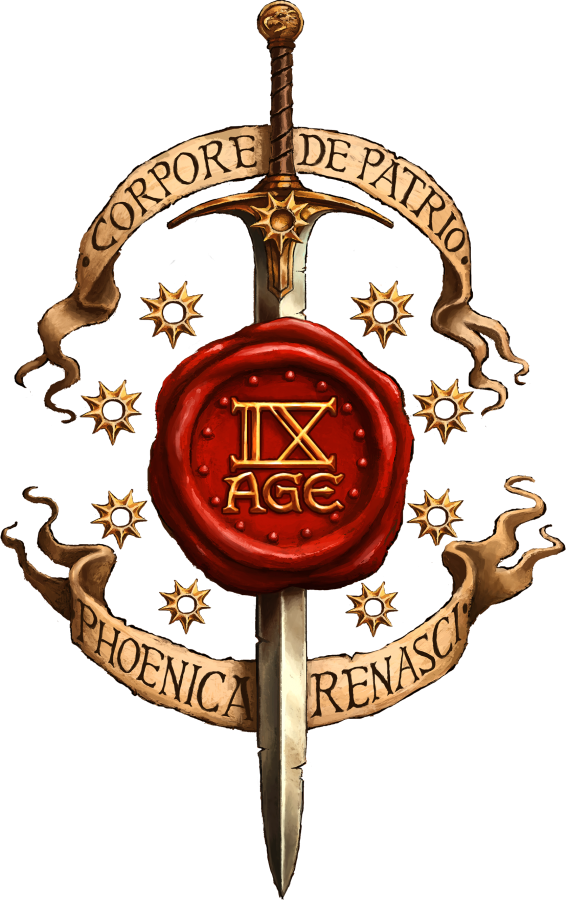
\includegraphics[height=10cm]{../Layout/pics/logo_9th.png}%
}

\vspace*{-1cm}
{\antiquefont\fontsize{50}{60}\selectfont \booktitle
\vspace{0.4cm}

\fontsize{14}{16.8}\selectfont \labels@armyrules{}

Beta v\version{} - \today{}}

\ifdef{\frenchversion}{{\fontsize{14}{16.8}\selectfont \vspace{0.2cm}\noindent\texttt{VF \frenchversion}}}{}
\vfill

\begin{tabular}{@{}m{2cm}@{\hskip 20pt}m{13cm}@{}}
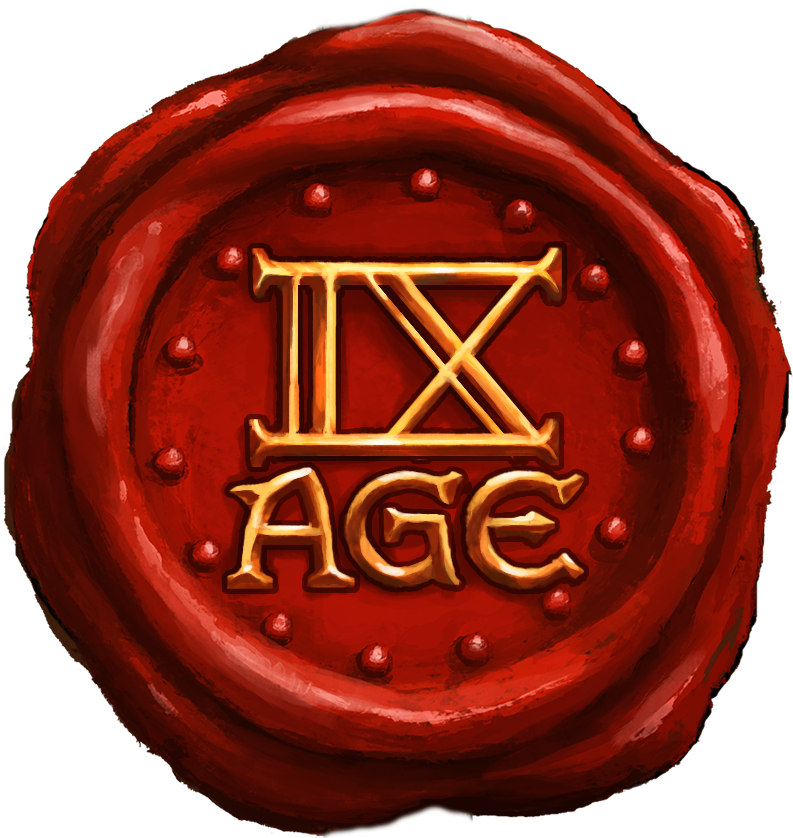
\includegraphics[width=2cm]{../Layout/pics/seal_9th.png} &
{\fontsize{10}{12}\selectfont \textcolor{black!50}{\noindent\labels@frontpagecredits}}

\ifdef{\frontpageaddstuff}{{\fontsize{10}{12}\selectfont \noindent\textcolor{black!50}{\frontpageaddstuff}}}{}

\vspace*{10pt}
\noindent{\fontsize{10}{12}\selectfont \textcolor{black!50}{\labels@license}}
\tabularnewline
\end{tabular}


\end{center}

\newpage

\thispagestyle{empty}

{\fontsize{10}{12}\selectfont

\ifdef{\labels@introduction}{\labels@introduction}{\vphantom{1pt}}
\vfill

\noindent\newrule{\labels@rulechanges}

\bigskip
\noindent \labels@latexcredit
}


\end{titlepage}

\restoregeometry

\startarmywiderules

\armyspecialruleentry{\risen{}}

Certains profils d'unité contiennent une catégorie appelée \risen{} qui donne le nombre de Points de Vie Ressuscités grâce à l'attribut \sandattribute{} de la Discipline \sands{}.

\armyspecialruleentry{\rulersofthedead{}}

Votre armée doit contenir au moins un Sorcier qui utilise la Discipline \sands{} que vous désignez comme étant votre Hiérophante. Il doit être indiqué sur votre liste d'armée. Le Hiérophante et toutes les figurines de son unité gagnent la règle \regeneration{6}.

\closearmywiderules








\vspace*{1.5cm}
\startarmyspecialrules

\armyspecialruleentry{\dusttodust{}}

À la fin de n'importe quelle phase durant laquelle le Hiérophante est retiré du jeu en tant que perte, toute unité de l'armée qui possède au moins une figurine avec la règle \dusttodust{} doit faire un test de Commandement. Si le test échoue, l'unité subit un nombre de blessures équivalent à la différence entre le résultat obtenu et la valeur de Commandement du test, sans aucune sauvegarde autorisée. Ces blessures sont réparties comme pour la règle \unstable{}, mais ne peuvent pas être assignées à une figurine n'ayant pas la règle \dusttodust{}. Le montant de blessures est réduit de un si l'unité est à portée de la règle \holdyourground{}.

À la fin du Tour de Joueur suivant la mort du Hiérophante, un nouveau Hiérophante peut être choisi. Pour ce faire, vous devez nommer un autre Personnage éligible, c'est à dire un Sorcier utilisant la Discipline \sands{}. Ce Personnage est le nouveau Hiérophante.

Au début de chacun de vos Tours de Joueur sans nouveau Hiérophante, toute unité qui possède au moins une figurine avec la règle \dusttodust{} doit faire un nouveau test de Commandement, et subir des blessures comme décrit ci-dessus.

\armyspecialruleentry{\undeadconstruct{}}

La figurine gagne les règles \dusttodust{} et \undead{}. Par ailleurs, une unité subit une blessure de moins lors de l'application de ces règles si au moins la moitié des figurines de l'unité possède la règle \undeadconstruct{}.

\armyspecialruleentry{\undyingwill{}}

Au début de n'importe quelle Phase de Corps à Corps, le Personnage peut conférer la valeur non modifiée de sa Capacité de Combat à toutes les figurines avec la règle \undead{} de son unité. S'il est monté sur une \largetarget{}, il peut à la place décider de conférer ce bonus à une unité alliée avec la règle \undead{} à moins de \distance{6}, à moins qu'il ne soit lui-même engagé au corps à corps. Dans ce dernier cas il ne peut conférer ce bonus qu'à une unité \undead{} engagée au corps à corps avec la même unité ennemie. Dans tous les cas, l'effet dure jusqu'à la fin de cette phase.

\armyspecialruleentry{\necromanticaura{}}

Toutes les unités alliées dans un rayon de \distance{6} d'une ou plusieurs figurines avec cette règle réduisent le nombre de blessures qu'elle subissent par les règles \dusttodust{} et \unstable{} de 1. Les figurines avec la règle \necromanticaura{} ne peuvent pas en bénéficier elles-mêmes.

\armyspecialruleentry{\mummyscurse{}}

Quand la figurine est retirée de la partie, la figurine qui lui a causé la blessure fatale subit une touche de Force 6 avec la règle \armourpiercing{6}. Si plusieurs figurines sont impliquées dans cette dernière blessure, déterminez aléatoirement qui est touché.

\armyspecialruleentry{\undergroundambush{}}

L'unité suit la règle \ambush{}. Cependant, au lieu d'entrer sur le champ de bataille à partir d'un bord de table, elle apparait à un endroit appelé le Point Souterrain. Au moment de le déterminer, le propriétaire commence par désigner un point à plus de \distance{3} de toute unité ennemie et à plus de \distance{0,5} de tout Terrain Infranchissable. Faites dévier ce point de \distance{2D6} pour obtenir le point souterrain. L'unité est alors placée avec le front du premier rang ou du rang arrière en contact avec le point souterrain. Si le point se trouve sous une unité ennemie, placez à la place l'unité embusquée en contact socle à socle avec le front avant de cette unité, en maximisant les figurines en contact comme en cas de charge. L'unité qui vient d'arriver est considérée comme ayant chargé et aucune réaction de charge ne peut être déclarée. S'il n'est pas possible de placer l'unité embusquée, considérez que le jet d'\ambush{} est raté et relancez le dé au prochain tour.

\closearmyspecialrules









\vspace*{1.5cm}
\startarmyarmoury

\startitemlistonecol

\listitemonecol{\aspenbow} Arme de Tir. \range{24}, Force 3, \volleyfire{}. Cette arme ignore tous les modificateurs pour toucher au tir.

\listitemonecol{\greataspenbow} Arme de Tir. \range{36}, Force 5, \volleyfire{}. Cette arme ignore tous les modificateurs pour toucher au tir. Compte comme une \hw{} avec -1 en Force au Corps à Corps.

\enditemlistonecol

\closearmyarmoury







\startarmynewsection{\monarchsofundead}

\spaceaftersection{}

\begin{center}
\noindent Ces options représentent des formes alternatives de l'armée que l'on peut rencontrer dans le vaste monde. Un \pharaoh{} peut décider de commander une des deux forces suivantes plutôt qu'une armée classique des Dynasties Immortelles.
\end{center}

\begin{multicols}{2}\raggedcolumns

\begin{center}\armynewsubsection{\commanderoftheterracottaarmy}\end{center} %M% vérifier les accords

\begin{itemize}[label={-}, leftmargin=*]
\item Tous les \skeletons{}, \skeletonarchers{}, la \skeletoncavalry{} et la \necropolisguard{} \textbf{doivent} être améliorés au coût de \pts{3}\permodel{} pour gagner +1 en Endurance, -1 en Initiative et la règle \undeadconstruct{}.

\item Une unité de \necropolisguard{} ne peut pas contenir plus de \textbf{30} figurines.

\item Toutes les autres unités n'ayant pas déjà la règle \undeadconstruct{}, y-compris les Personnages, \textbf{doivent} être améliorés au coût de \pts{15}\permodel{} pour gagner +1 en Endurance, -1 en Initiative et la règle \undeadconstruct{}. Elles perdent la règle \flammable{} si elles l'avaient.

\item Une unité de \skeletonchariots{} ne peut pas contenir plus de \textbf{6} figurines.

\item La caractéristique \risen{} de toutes les figurines est fixée à 1.

\item Les figurines non volantes qui possèdent la ou les règles \undergroundambush{} ou \lighttroops{} les perdent, et ne peuvent en aucun cas gagner ces règles.

\item Les \greatvultures{}, \scarabswarms{} et \wingedreapers{} ne peuvent pas être pris dans cette armée.
\end{itemize}

\vspace*{\fill}\columnbreak

\begin{center}\armynewsubsection{\lordofthebarrowlegion}\end{center}

\begin{itemize}[label={-}, leftmargin=*]
\item Les \skeletons{} et \skeletonarchers{} \textbf{doivent} prendre une \ha{} pour \pts{2}\permodel{}

\item Les \skeletons{} peuvent échanger la \spear{} et le \shield{} contre une \halberd{} pour \pts{1}\permodel{}

\item La \skeletoncavalry{} peut disposer d'une \lance{} pour \pts{3}\permodel{} et d'un \barding{} pour \pts{3}\permodel{}

\item Les \skeletonchariots{} \textbf{doivent} prendre une \ha{} pour \pts{5}\permodel{} et peuvent prendre une \halberd{} pour \pts{5}\permodel{} Une unité de \skeletonchariots{} ne peut pas contenir plus de \textbf{7} figurines.

\item La \necropolisguard{} doit prendre une \ha{} pour \pts{2}\permodel{} Une unité de \necropolisguard{} ne peut pas contenir plus de \textbf{35} figurines.

\item Les \scarabswarms{} doivent gagner la règle \ethereal{} pour \pts{15}\permodel{} Une unité de \scarabswarms{} ne peut pas contenir plus de \textbf{4} figurines.

\item La caractéristique \risen{} des figurines avec la règle \ethereal{} est fixée à 1.

\item Les figurines de \monstrouscavalry{} ou avec la règle \largetarget{} ne peuvent pas être prises dans cette armée.

\item Les figurines qui possèdent la ou les règles \undergroundambush{} ou \scout{} les perdent, et ne peuvent en aucun cas gagner ces règles.

\item Les figurines non volantes qui possèdent une \ha{} et la règle \lighttroops{} perdent cette règle, et ne peuvent en aucun cas la regagner.
\end{itemize}

\vspace*{\fill}\end{multicols}

\closearmynewsection








\startarmymagicalitems

\armymagicalweapons

\startpricelist

\pricelistitem{L'Éternel Vainqueur}{55}Figurine à pied uniquement.

 Type : \halberd{}. Les attaques portées avec cette arme possèdent la règle \lethalstrike{}. Le porteur peut utiliser l'arme de deux manières : Attaque Ciblée ou Attaque Faucheuse. Choisissez au début de chaque Manche de Corps à Corps.
 \begin{itemize}[label={-}]
\item \textbf{Attaque Ciblée} : Les attaques portées avec cette arme gagnent la règle \multiplewounds{1D3}{}.
\item \textbf{Attaque Faucheuse} : Toutes les attaques du porteur sont échangées contre une touche automatique à chaque figurine en contact socle à socle avec le porteur. Toutes les figurines qui peuvent effectuer une attaque de soutien contre le porteur subissent aussi une attaque qui touche sur 4+. Ces attaques suivent les règles normales de l'arme (\halberd{}, \lethalstrike{}).
\end{itemize}
%M% strike plutôt coup que attaque

\pricelistitem{Fléau des Rois}{50/30} Type : \hw{}. Les attaques effectuées avec cette arme possèdent la règle \armourpiercing{1}. Chaque touche réussie avec cette arme occasionne deux touches.

\endpricelist

\armymagicalarmour

\startpricelist

\pricelistitem{Couronne des Pharaons}{45} Type : Aucun (Sauvegarde d'Armure 6+). Le porteur peut utiliser la règle \undyingwill{} sur une seule unité alliée à moins de \distance{6}. Si le porteur est engagé au corps à corps, il ne peut transférer sa Capacité de Combat non modifiée qu'à une unité avec la règle \undead{} alliée au corps à corps avec la même unité ennemie. De plus, vous pouvez choisir d'utiliser la règle \undyingwill{} durant la Phase de Tir en transférant sa Capacité de Tir à la place de sa Capacité de Combat. La règle \undyingwill{} ne peut être utilisée que lors d'une seule phase par Tour de Joueur. Si le porteur est monté sur une \largetarget{}, ajoutez \distance{6} à la portée de l'objet.

\pricelistitem{Armure des Éternités}{35}Figurine à pied uniquement.

Type : \platearmour{}. Le porteur gagne +1 Point de Vie.

\endpricelist

\armytalismans

\startpricelist

\pricelistitem{Broche Solaire}{15} Au début de chaque Manche de Corps à Corps, choisissez un élément de figurine en contact socle à socle avec le porteur. Il subit un malus de -1 sur sa caractéristique Attaque, jusqu'à un minimum de 1.

\endpricelist

\armyenchanteditems

\startpricelist

\pricelistitem{Masque de Mort de Teput}{35} Au début de chaque Manche de Corps à Corps, choisissez la règle \inspiringpresence{} ou \holdyourground{}. Les unités ennemies en contact socle à socle avec le porteur ne peuvent plus bénéficier de la règle choisie pour la durée de cette phase.
%M% mortuaire ?

\pricelistitem{Cape des Tempêtes de Sable}{30} L'unité du porteur gagne la règle \hardtarget{}.

\pricelistitem{Char Solaire de Nephet-Râ}{25} Figurine sur \chariot{} uniquement.

Les \impacthits{} causées par le \chariot{} du porteur et les Attaques de ses montures gagnent les règles \flamingattacks{} et \magicalattacks{} et sont résolues avec +1 en Force.

\endpricelist

\armyarcaneitems

\startpricelist

\pricelistitem{Livre des Morts}{50/35} La valeur de lancement des sorts de la Discipline \sands{} est réduite de 1 pour le porteur. De plus, l'Attribut de la Discipline \sands{} lancé par le porteur Ressuscite 1 PV supplémentaire sur la ou les unités ciblées qui ne sont ni des Personnages ni des Grandes Cibles.

\endpricelist

\armymagicalbanners

\startpricelist

\pricelistitem{Bannière des Ensablés}{65} Les figurines avec la règle \undergroundambush{} de l'armée peuvent ajouter +1 à leur jet d'\ambush{}. Signalez-le avant de lancer le dé. Si vous utilisez ce bonus, le point souterrain doit se trouver à moins de \distance{24} du porteur et ne dévie que de \distance{1D6}.

\endpricelist

\closearmymagicalitems








%%% START OF THE ARMYLIST - Translators shouldn't have to edit it %%%

%\armylist

\lordstitle

\showunit{
	name={\pharaoh},
	cost=160,
	profile={< 4 6 3 5 5 4 3 4 10},
	type=\infantry{},
	unitsize=1,
	invocation=1,
	basesize=20x20,
	commontype=\undeadcommonrules{},
	commonspecialrules={\undead{},\dusttodust{}},
	specialrules={\mummyscurse{},\flammable{},\fear{},\undyingwill{}},
	armour={\la},
	options={
		\magicalitemsallowance{}=\upto{}<100,
		\shield{}=3,
		\ha{}=12,
		\greataspenbow{}=10,
		\weapononechoice{
			\flail{}=5,
			\pw{}=5,
			\halberd{}=10,
			\gw{}=15,
			\lance{}=15,
		},
		\onechoiceonly{} \only{\general}{
			\commanderoftheterracottaarmy{}=\free{},
			\lordofthebarrowlegion{}=\free{},
		},
	}
	mounts={\skeletalhorse{}=20,\skeletonchariot{}=35,\royalsphinx{}=185},
}
	
\showunit{
	name={\deathculthierarch},
	cost=170,
	profile={< 4 3 3 3 4 3 2 1 8},
	type=\infantry{},
	unitsize=1,
	invocation=1,
	basesize=20x20,
	commontype=\undeadcommonrules{},
	commonspecialrules={\undead{},\dusttodust{}},
	magiclevel=3,
	magicpaths={\light{},\death{},\sands},
	options={
		\magiclevel{4}=30,
		\soulconduit{}=50,
		\magicalitemsallowance{}=\upto{}<100,
		},
	mounts={\skeletalhorse{}=20,\arkofages{}=170},
	unitrules={
		\unitrule{\soulconduit{}}{\soulconduitrule{}}
		},	
}
		






\heroestitle	

%\showunit{
%	name={\nomarch{}},
%	cost={100},
%	profile={< 4 5 3 4 5 3 3 3 9},
%	type=\infantry{},
%	unitsize={1},
%	invocation={1},
%	basesize=20x20,
%	commontype=\undeadcommonrules{},
%	commonspecialrules={\undead{}, \dusttodust{}},
%	specialrules={\mummyscurse{}, \undyingwill{}, \flammable{}, \fear{}},
%	armour={\la{}},
%	options={
%		\magicalitemsallowance{}=\upto{}<50,
%		\shield{}=3
%		\ha{}=12,
%		\aspenbow{}=3,
%		\weapononechoice
%			{
%			\pw{}=3,
%			\flail{}=3,
%			\halberd{}=4,
%			\lance{}=6,
%			\gw{}=6,
%			}
%		}
%	mounts={\skeletalhorse{}=20,\skeletonchariot{}=35,\royalsphinx{}=200},
%}
%
%	
%\showunit{
%	name={\deathcultaccolyte{}},
%	cost={65},
%	profile={< 4 3 3 3 3 2 2 1 7},
%	type=\infantry{},
%	unitsize={1},
%	invocation={1},
%	basesize=20x20,
%	commontype=\undeadcommonrules{},
%	commonspecialrules={\undead{},\dusttodust{}},
%	magiclevel=1,
%	magicpaths={\light, \death, \sands},
%	options={
%		\magicalitemsallowance{}=\upto{}<50,
%		\magiclevel{2}=25,
%		},
%	mounts={\skeletalhorse{}=15,\arkofages{}=180},
%}
%	
%\showunit{
%	name={\tombharbinger{}},
%	cost={70},
%	profile={< 4 4 3 4 5 2 3 3 8},
%	type=\infantry{},
%	unitsize={1},
%	invocation={1},
%	basesize=20x20,
%	commontype=\undeadcommonrules{},
%	commonspecialrules={\undead{}, \dusttodust{}},
%	specialrules={\poisonedattacks{}, \lethalstrike{}, \flammable{}, \guardianswrath{}, \royalguard{}},
%	armour={\la{}},
%	options={
%		\bsb{}=25,
%		\magicalitemsallowance{}=\upto{}<50,
%		\shield{}=3
%		\ha{}=12,
%		\aspenbow{}=3,
%		\weapononechoice
%			{
%			\pw{}=3,
%			\flail{}=3,
%			\halberd{}=4,
%			\lance{}=6,
%			\gw{}=6,
%			},
%		}
%	mounts={\skeletalhorse{}=20,\skeletonchariot{}=50,\amuut{}=50},
%	unitrules={
%		\unitrule{\guardianswrath{}}{\guardianswrathrule{}}
%		\unitrule{\royalguard{}}{\royalguardrule{}}
%		},	
%}
%
%\showunit{
%	name={\tombarchitect{}},
%	cost={50},
%	profile={< 4 4 3 4 4 2 3 2 7},
%	type=\infantry{},
%	unitsize={1},
%	invocation={1},
%	basesize=20x20,
%	commontype=\undeadcommonrules{},
%	commonspecialrules={\undead{}, \dusttodust{}},
%	specialrules={\flammable{}, \masterofstone{}, \masonsmenagerie{}},
%	armour={\la{}},
%	options={
%		\magicalitemsallowance{}=\upto{}<50,
%		\weapononechoice
%			{
%			\pw{}=3,
%			\lance{}=6,
%			},
%		\mastermason{}=25,		
%		}
%	mounts={\skeletalhorse{}=15,\skeletonchariot{}=50,\amuut{}=50},
%	unitrules={
%		\unitrule{\masonsmenagerie{}}{\masonsmenagerierule{}}
%		\unitrule{\masterofstone{}}{\masterofstonerule{}}
%		\unitrule{\mastermason{}}{\mastermasonrule{}}
%		},	
%}








\mountstitle

%\showunit{
%	name={\skeletalhorse{}},
%	profile={< 8 2 - 3 3 1 2 1 3},
%	type=\warbeast{},
%	basesize=25x50,
%	armour={\mountsprotection{6}},
%	options={
%			\barding{}=10
%		}, 		
%	}
%	
%\showunit{
%	name={\amuut{}},
%	profile={< 7 3 - 5 4 3 3 3 8},
%	type=\monstrousbeast{},
%	basesize=50x100,
%	commontype=\undeadcommonrules{},
%	commonspecialrules={\undeadconstruct{}},
%	specialrules={\poisonedattacks{}, \fear{}},
%	armour={\mountsprotection{6}},
%		}
%	
%\showunit{
%	name={\royalsphinx{}},
%	profile={< 6 4 - 5 6 5 1 4 8},
%	type=\monstrousbeast{},
%	basesize=50x100,
%	commontype=\undeadcommonrules{},
%	commonspecialrules={\undeadconstruct{}},
%	specialrules={\poisonedattacks{}, \largetarget{}, \stomp{1D6}, \terror{}},
%	options={
%			\necromanticaura{}=15,
%			\lethalstrike{}=25,
%			}, 		
%	}
%	
%\showunit{
%	name={\skeletonchariot{}},
%	profile={
%	\skeletonchariot{}< - - - 4 4 3 - - -,
%	\skeletalhorse{}(2)< 8 2 - 3 - - 2 1 -,
%	},
%	type=\chariot{},
%	basesize=50x100,
%	armour={\mountsprotection{6}},
%	options={
%			\twoadditionalhorses{}=\free,
%			}, 		
%	}
%	
%\showunit{
%	name={\arkofages{}},
%	profile={
%	\arkofages{}< - - - 4 5 5 - - -,
%	\guard{}(2)< - 3 3 4 - - 3 1 8,
%	\boundspirits{}(1)< 4 2 - 2 - - 2 6 -,
%	},
%	type=\chariot{},
%	basesize=60x100,
%	commontype=\undeadcommonrules{},
%	commonspecialrules={\undeadconstruct{}},
%	specialrules={\poisonedattacks{}\only{\guard{}}, \magicalattacks{}, \lethalstrike{}\only{\guard{}}, \warplatform{}, \wardsave{5}, \divineprotection{}, \sacredark{}},
%	armour={\mountsprotection{5}},
%	weapons={\aspenbow{}\only{\guard{}}}
%	options={
%			\necromanticaura{}=15,
%			}, 	
%	unitrules={
%		\unitrule{\sacredark{}}{\sacredarkrule{}}
%		\unitrule{\divineprotection{}}{\divineprotectionrule{}}
%		},				
%	}	








\coreunitstitle		
	
%\showunit{
%	name={\skeletons{}},
%	QRSname={\skeleton{}},
%	cost={80},
%	profile={< 4 2 2 3 3 1 2 1 4},
%	type=\infantry{},
%	invocation={1D3+3},
%	unitsize=20,
%	maxmodels=60,
%	costpermodel=5,
%	basesize=20x20,
%	commontype=\undeadcommonrules{},
%	commonspecialrules={\undead{},\dusttodust{}},
%	armour={\la{},\shield{}},
%	options={
%		\spear{}=\free,
%	},
%	commandgroup={champion=10, musician=10, banner=10, veteranstandardbearer=yessir},
%}
%
%\showunit{
%	name={\skeletonarchers{}},
%	QRSname={\skeletonarcher{}},
%	cost={60},
%	profile={< 4 2 2 3 3 1 2 1 4},
%	type=\infantry{},
%	invocation={1D3+3},
%	unitsize=10,
%	maxmodels=30,
%	costpermodel=6,
%	basesize=20x20,
%	commontype=\undeadcommonrules{},
%	commonspecialrules={\undead{},\dusttodust{}},
%	weapons={\aspenbow{}},
%	armour={\la{}},
%	commandgroup={champion=10, musician=10, banner=10, veteranstandardbearer=yessir},
%}
%
%\showunit{
%	name={\skeletoncavalry{}},
%	cost={65},
%	profile={
%		\rider{}< 4 3 2 3 3 1 2 1 6,
%		\skeletalhorse{}< 8 2 - 3 3 1 2 1 3,
%	},
%	type=\cavalry{},
%	invocation={1D3+2},
%	unitsize=5,
%	maxmodels=20,
%	costpermodel=11,
%	basesize=25x50,
%	commontype=\undeadcommonrules{},
%	commonspecialrules={\undead{},\dusttodust{}},
%	specialrules={\vanguard{},\scout{},\lighttroops{}},
%	armour={\shield{},\mountsprotection{6}},
%	options={
%		\exchangescoutandlighttroopsforla{}=\permodel{}<1,
%		\onechoiceonly{
%			\exchangeshieldandvanguardforaspenbow{}=\free{},
%			\lightlance{}=\permodel{}<1,
%		},
%	},
%	commandgroup={champion=10, musician=10, banner=10, veteranstandardbearer=yessir},
%}
%
%\showunit{
%	name={\skeletonchariots{}},
%	cost={135},
%	profile={
%		\chariot{}< - - - 4 4 3 - - -,
%		\charioteer{} (2)< - 3 2 3 - - 2 2 7,
%		\skeletalhorse{} (2)< 8 2 - 3 - - 2 1 -,
%	},
%	type=\chariot{},
%	invocation={1D3+1},
%	unitsize=5,
%	maxmodels=10,
%	costpermodel=35,
%	basesize=50x100,
%	commontype=\undeadcommonrules{},
%	commonspecialrules={\undead{},\dusttodust{}},
%	weapons={\aspenbow{} \only{\charioteer{}},\lightlance{} \only{\charioteer{}}},
%	armour={\la{},\mountsprotection{6}},
%	options={
%		\lighttroops{}=\free{},
%	},
%	commandgroup={champion=10, musician=10, banner=10, veteranstandardbearer=yessir},
%}









\specialunitstitle

%\showunit{
%	name={\necropolisguard{}},
%	cost={70},
%	profile={< 4 3 3 4 4 1 3 1 8},
%	type=\infantry{},
%	invocation={1D3+1},
%	unitsize=10,
%	maxmodels=40,
%	costpermodel=11,
%	basesize=20x20,
%	commontype=\undeadcommonrules{},
%	commonspecialrules={\undead{},\dusttodust{}},
%	specialrules={\lethalstrike{},\bodyguard{},\magicalattacks{},\poisonedattacks{}},
%	armour={\la{}},
%	options={
%		\shield{}=\permodel{}<1,
%		\onechoiceonly{
%			\pw{}=\permodel{}<1,
%			\halberd{}=\permodel{}<2,
%		},
%	},
%	commandgroup={champion=10, musician=10, banner=10, bannerallowance=50},
%}
%
%\showunit{
%	name={\scarabswarms{}},
%	QRSname={\scarabswarm{}},
%	cost={70},
%	profile={< 5 3 - 2 2 5 1 5 10},
%	type=\swarm{},
%	invocation={1D3+3},
%	unitsize=2,
%	maxmodels=7,
%	costpermodel=25,
%	basesize=40x40,
%	commontype=\undeadcommonrules{},
%	commonspecialrules={\undead{},\dusttodust{}},
%	specialrules={\armourpiercing{1},\poisonedattacks{}\hardtarget{},\distracting{},\undergroundambush{}},
%}
%
%\showunit{
%	name={\shabtis{}},
%	QRSname={\shabti{}},
%	cost={100},
%	profile={< 6 4 2 5 4 3 3 3 8},
%	type=\monstrousinfantry{},
%	invocation={1},
%	unitsize=3,
%	maxmodels=10,
%	costpermodel=37,
%	basesize=40x40,
%	commontype=\undeadcommonrules{},
%	commonspecialrules={\undeadconstruct{}},
%	specialrules={\fear{}},
%	armour={\la{},\innatedefence{5}},
%	options={
%		\weapononechoice{
%			\greataspenbow{}=\free{},
%			\pw{}=\permodel{}<5,
%			\halberd{}=\permodel{}10,
%		}
%	},
%	commandgroup={champion=10, musician=10, banner=10, bannerallowance=25},
%}
%
%\showunit{
%	name={\tombcataphracts{}},
%	QRSname={\tombcataphract{}},
%	cost={165},
%	profile={
%		\rider{}< 4 4 3 4 4 1 3 2 8,
%		\amuut{}< 7 3 - 5 4 3 3 3 8,
%	},
%	type=\monstrouscavalry{},
%	invocation={1},
%	unitsize=3,
%	maxmodels=6,
%	costpermodel=55,
%	basesize=50x100,
%	commontype=\undeadcommonrules{},
%	commonspecialrules={\undeadconstruct{}},
%	specialrules={\fear{},\lethalstrike{} \only{\rider{}},\poisonedattacks{} \only{\amuut{}}},
%	weapons={\lightlance{} \only{\rider{}}},
%	armour={\la{},\innatedefence{5}, \mountsprotection{6}},
%	options={
%		\undergroundambush{}=20,
%		}
%	},
%	commandgroup={champion=10, musician=10, banner=10, bannerallowance=50},
%}
%
%\showunit{
%	name={\greatvultures{}},
%	QRSname={\greatvulture{}},
%	cost={80},
%	profile={< 2 3 - 4 4 2 3 3 4},
%	type=\warbeast{},
%	invocation={1D3+1},
%	unitsize=3,
%	maxmodels=9,
%	costpermodel=20,
%	basesize=40x40,
%	commontype=\undeadcommonrules{},
%	commonspecialrules={\undead{},\dusttodust{}},
%	specialrules={\fly{9},\skirmisher{}},
%}
%
%\showunit{
%	name={\sandscorpion{}},
%	cost={85},
%	profile={< 7 4 - 5 5 4 3 4 8},
%	type=\monstrousbeast{},
%	invocation={1},
%	unitsize=1,
%	basesize=50x50,
%	commontype=\undeadcommonrules{},
%	commonspecialrules={\undeadconstruct{}},
%	specialrules={\fear{},\lethalstrike{},\poisonedattacks{},\magicresistance{2},\undergroundambush{}},
%	armour={\innatedefence{5}},
%}
%
%\showunit{
%	name={\sandstalkers{}},
%	QRSname={\sandstalker{}},
%	cost={165},
%	profile={< 7 3 5 4 4 3 3 2 8},
%	type=\monstrousbeast{},
%	invocation={1},
%	unitsize=3,
%	maxmodels=7,
%	costpermodel=50,
%	basesize=50x100,
%	commontype=\undeadcommonrules{},
%	commonspecialrules={\undeadconstruct{}},
%	specialrules={\fear{},\lighttroops{}},
%	weapons={\halberd{}},
%	armour={\innatedefence{5}},
%	options={
%		\undergroundambush{}=20,
%		}
%	},
%	commandgroup={champion=10},
%	unitequipment={\equipmentdef{\petrifyinggaze{}}{\petrifyinggazerule{}}},
%}
%
%\showunit{
%	name={\battlesphinx{}},
%	cost={220},
%	profile={
%		\battlesphinx{}< 6 4 - 5 8 5 1 4 8,
%		\rider{} (4)< - 4 3 4 - - 3 2 8,
%	},
%	type=\riddenmonster{},
%	invocation={1},
%	unitsize=1,
%	basesize=50x100,
%	commontype=\undeadcommonrules{},
%	commonspecialrules={\undeadconstruct{}},
%	specialrules={\lethalstrike{} \only{\rider{}},\poisonedattacks{} \only{\battlesphinx{}}},
%	weapons={\lightlance{} \only{\rider{}}},
%	armour={\innatedefence{5}},
%	options={
%		\innatedefence{4}=25,
%		\breathweaponbattlesphinx{}=25,
%	},
%}








\rareunitstitle

%\showunit{
%	name={\wingedreapers{}},
%	QRSname={\wingedreaper{}},
%	cost={155},
%	profile={< 6 5 3 5 5 4 4 4 10},
%	type=\monstrousinfantry{},
%	invocation={1},
%	unitsize=2,
%	maxmodels=5,
%	costpermodel=72,
%	basesize=50x75,
%	commontype=\undeadcommonrules{},
%	commonspecialrules={\undeadconstruct{}},
%	specialrules={\fear{},\fly{6},\lethalstrike{}},
%	armour={\innatedefence{5}},
%	options={
%		\onechoiceonly{
%			\autonomous{}=\permodel{}<10,
%			\necromanticaura{}=20,
%		},
%		\la{}=\permodel{}<10,
%		\weapononechoice{
%			\pw{}=\permodel{}<5,
%			\halberd{}=\permodel{}12,
%		}
%	},
%	unitrules={\unitrule{\autonomous{}}{\autonomous{}}},
%}
%
%\showunit{
%	name={\dreadsphinx{}},
%	cost={245},
%	profile={< 6 5 - 6 8 5 1 4 8},
%	type=\monster{},
%	invocation={1},
%	unitsize=1,
%	basesize=50x100,
%	commontype=\undeadcommonrules{},
%	commonspecialrules={\undeadconstruct{}},
%	specialrules={\fly{6},\lethalstrike{},\poisonedattacks{},\multiplewounds{2}{\monster{},\riddenmonster{}}},
%	weapons={\pw{}},
%	armour={\innatedefence{5}},
%	options={
%		\innatedefence{4}=25,
%	},
%}
%
%\showunit{
%	name={\colossus{}},
%	cost={195},
%	profile={< 6 4 2 6 6 5 2 5 8},
%	type=\monster{},
%	invocation={1},
%	unitsize=1,
%	basesize=50x50,
%	commontype=\undeadcommonrules{},
%	commonspecialrules={\undeadconstruct{}},
%	specialrules={\grindingattacks{1D3+1}},
%	armour={\la{},\innatedefence{5}},
%	options={
%		\weapononechoice{
%			\scalesofdestiny{}=5,
%			\pw{}=10,
%			\gw{}=20,
%			\giantaspenbow{}=10,
%		},
%	},
%	unitrules={
%		\unitrule{\scalesofdestiny{}}{\scalesofdestinyrule{}}
%		\unitrule{\giantaspenbow{}}{\giantaspenbowrule{}}
%	},
%}
%
%\showunit{
%	name={\casketofphatep{}},
%	cost={115},
%	profile={
%		\casket{}< - - - - 7 3 - - -,
%		\necropolisguard{} (3)< 4 3 3 4 4 - 3 1 8,
%	},
%	type=\warmachine{},
%	invocation={1},
%	unitsize=1,
%	basesize=75,
%	commontype=\undeadcommonrules{},
%	commonspecialrules={\undead{},\dusttodust{}},
%	specialrules={\lethalstrike{} \only{\necropolisguard{}},\poisonedattacks{} \only{\necropolisguard{}},\magicalattacks{},\wardsave{5},\divinelight{},\phatepscurse{}},
%	weapons={\halberd{} \only{\necropolisguard{}}},
%	armour={\la{}},
%	unitrules={
%		\unitrule{\divinelight{}}{\divinelightrule{}}
%		\unitrule{\phatepscurse{}}{\phatepscurserule{}}
%	},
%}
%
%\showunit{
%	name={\charnelcatapult{}},
%	cost={90},
%	profile={
%		\charnelcatapult{}< - - - - 7 3 - - -,
%		\skeleton{} (3)< 4 2 2 3 3 - 2 1 4,
%	},
%	type=\warmachine{},
%	invocation={1},
%	unitsize=1,
%	basesize=75,
%	commontype=\undeadcommonrules{},
%	commonspecialrules={\undead{},\dusttodust{}},
%	unitrules={\unitrule{\cursedammunition{}}{\cursedammunitionrule{}}},
%	unitequipment={\equipmentdef{\charnelcatapult{}}{\charnelcatapultrule{}}},
%	options={
%		\replacecharnelcatapultwithcursedammunition{}=35
%	},
%}



%%% Quick Reference Sheet - AB_qrs.tex is automatic and shouldn't be edited %%%

\quickrefsheettitle

% Script to automatically draw the Quick Ref Sheet

\renewcommand{\arraystretch}{1.2}

\providebool{QRSbool}

\providebool{whiterow}

\newcommand{\QRSrowcolor}{\ifbool{whiterow}{\global\boolfalse{whiterow}}{\rowcolor{black!10}\global\booltrue{whiterow}}}

\newcommand{\QRSstarttab}[1]{%
	\noindent%
	\setlength{\tabcolsep}{2pt}%
	\begin{tabular}{@{}cp{3.2cm}M{\profilecellsize}@{}M{\profilecellsize}@{}M{\profilecellsize}@{}M{\profilecellsize}@{}M{\profilecellsize}@{}M{\profilecellsize}@{}M{\profilecellsize}@{}M{\profilecellsize}@{}M{\profilecellsize}}%

	& \antiquefont\large{\textbf{#1}} & \textbf{\labels@M} & \textbf{\labels@WS} & \textbf{\labels@BS} & \textbf{\labels@S} & \textbf{\labels@T} & \textbf{\labels@W} & \textbf{\labels@I} & \textbf{\labels@A} & \textbf{\labels@Ld}%
}%

\newcommand{\QRSclosetab}{\end{tabular}\bigskip}%

\newcommand{\QRSprintline}[4]{%
	\tabularnewline%
	\ifnumequal{\rowmulti}{1}{\QRSrowcolor}{}%
	\DTLifeq*{\rowcategory}{\labels@lords}{\antiquefont\bfseries \labels@lordsInitial}{}%
	\DTLifeq*{\rowcategory}{\labels@heroes}{\antiquefont\bfseries \labels@heroesInitial}{}%
	\DTLifeq*{\rowcategory}{\labels@coreunits}{\antiquefont\bfseries \labels@coreunitsInitial}{}%
	\DTLifeq*{\rowcategory}{\labels@specialunits}{\antiquefont\bfseries \labels@specialunitsInitial}{}%
	\DTLifeq*{\rowcategory}{\labels@rareunits}{\antiquefont\bfseries \labels@rareunitsInitial}{}%
	\DTLifeq*{\rowcategory}{\labels@mounts}{\antiquefont\bfseries \labels@mountsInitial}{}%
	&%
	\ifnumequal{\rowmulti}{1}{%no Multiprofile
		\rowname%
		\expandafter\parselist\expandafter{\rowprofile}{\locallists@profileslist}%
		\forlistloop{\QRSmonoprofile}{\locallists@profileslist}%
	}{% Multiprofile
		\rowname &&&&&&&&&%
		\expandafter\parselist\expandafter{\rowprofile}{\locallists@profileslist}%
		\forlistloop{\QRSmultiprofile}{\locallists@profileslist}%
	}%
}

\newcommand{\QRSmultiprofile}[1]{%
	\tabularnewline%
	\QRSrowcolor{}&%
	\splitatinf{#1}\local@unitname\local@unitprofile%
	- \local@unitname \expandafter\caraclist\expandafter{\local@unitprofile}%
}%

\newcommand{\QRSmonoprofile}[1]{%
	\splitatinf{#1}\local@unitname\local@unitprofile%
	\expandafter\caraclist\expandafter{\local@unitprofile}%
}%

\newcommand{\QRSprinttab}[1]{%
	\global\booltrue{whiterow}%
	\DTLforeach*[#1]%
	{profiles}{\rowname=name, \rowtrooptype=trooptype, \rowcategory=category, \rowprofile=profile, \rowmulti=multipleprofile}{%
      		\QRSprintline{\rowname}{\rowcategory}{\rowprofile}{\rowmulti}%
	}%
}%

\providebool{QRSisempty}
\global\boolfalse{QRSisempty}%

\newcommand{\QRScheckifempty}[1]{%
	\global\booltrue{QRSisempty}%
	\DTLforeach*[#1]%
	{profiles}{\rowname=name, \rowtrooptype=trooptype, \rowcategory=category, \rowprofile=profile, \rowmulti=multipleprofile}{%
		\global\boolfalse{QRSisempty}\dtlbreak%
	}%
}%

\newcommand{\QRSifnotempty}[1]{%
	\ifbool{QRSisempty}{}{#1}%
}%

\begin{center}
{\antiquefont\bfseries \labels@lordsInitial}\spacebeforecolon{}: \labels@lords{} - %
{\antiquefont\bfseries \labels@heroesInitial}\spacebeforecolon{}: \labels@heroes{} - %
{\antiquefont\bfseries \labels@coreunitsInitial}\spacebeforecolon{}: \labels@coreunits{} - %
{\antiquefont\bfseries \labels@specialunitsInitial}\spacebeforecolon{}: \labels@specialunits{} - %
{\antiquefont\bfseries \labels@rareunitsInitial}\spacebeforecolon{}: \labels@rareunits{} - %
{\antiquefont\bfseries \labels@mountsInitial}\spacebeforecolon{}: \labels@mounts{}%
\end{center}

\begin{multicols}{2}

\QRScheckifempty{%
	\DTLiseq{\rowcategory}{\labels@lords}\or\DTLiseq{\rowcategory}{\labels@heroes}%
}%
\QRSifnotempty{%
	\QRSstarttab{\characters}%
	\QRSprinttab{%
		\DTLiseq{\rowcategory}{\labels@lords}\or\DTLiseq{\rowcategory}{\labels@heroes}%
	}%
	\QRSclosetab{}%
}%

\QRScheckifempty{%
	\DTLiseq{\rowtrooptype}{\infantry}\and\not\DTLiseq{\rowcategory}{\labels@heroes}\and\not\DTLiseq{\rowcategory}{\labels@lords}%
}%
\QRSifnotempty{%
	\QRSstarttab{\infantry}%
	\QRSprinttab{%
		\DTLiseq{\rowtrooptype}{\infantry}\and\not\DTLiseq{\rowcategory}{\labels@heroes}\and\not\DTLiseq{\rowcategory}{\labels@lords}%
	}% 
	\QRSclosetab{}%
}% 

\QRScheckifempty{%
	\DTLiseq{\rowtrooptype}{\monstrousinfantry}\and\not\DTLiseq{\rowcategory}{\labels@heroes}\and\not\DTLiseq{\rowcategory}{\labels@lords}%
}%
\QRSifnotempty{%
	\QRSstarttab{\monstrousinfantry}%
	\QRSprinttab{%
		\DTLiseq{\rowtrooptype}{\monstrousinfantry}\and\not\DTLiseq{\rowcategory}{\labels@heroes}\and\not\DTLiseq{\rowcategory}{\labels@lords}%
	}% 
	\QRSclosetab{}%
}% 

\QRScheckifempty{%
	\DTLiseq{\rowtrooptype}{\warbeast}\and\not\DTLiseq{\rowcategory}{\labels@heroes}\and\not\DTLiseq{\rowcategory}{\labels@lords}%
}%
\QRSifnotempty{%
	\QRSstarttab{\warbeasts}%
	\QRSprinttab{%
		\DTLiseq{\rowtrooptype}{\warbeast}\and\not\DTLiseq{\rowcategory}{\labels@heroes}\and\not\DTLiseq{\rowcategory}{\labels@lords}%
	}% 
	\QRSclosetab{}%
}% 

\QRScheckifempty{%
	\DTLiseq{\rowtrooptype}{\monstrousbeast}\and\not\DTLiseq{\rowcategory}{\labels@heroes}\and\not\DTLiseq{\rowcategory}{\labels@lords}%
}%
\QRSifnotempty{%
	\QRSstarttab{\monstrousbeasts}%
	\QRSprinttab{%
		\DTLiseq{\rowtrooptype}{\monstrousbeast}\and\not\DTLiseq{\rowcategory}{\labels@heroes}\and\not\DTLiseq{\rowcategory}{\labels@lords}%
	}% 
	\QRSclosetab{}%
}% 

\QRScheckifempty{%
	\DTLiseq{\rowtrooptype}{\cavalry}\and\not\DTLiseq{\rowcategory}{\labels@heroes}\and\not\DTLiseq{\rowcategory}{\labels@lords}%
}%
\QRSifnotempty{%
	\QRSstarttab{\cavalry}%
	\QRSprinttab{%
		\DTLiseq{\rowtrooptype}{\cavalry}\and\not\DTLiseq{\rowcategory}{\labels@heroes}\and\not\DTLiseq{\rowcategory}{\labels@lords}%
	}%
	\QRSclosetab{}%
}% 

\QRScheckifempty{%
	\DTLiseq{\rowtrooptype}{\monstrouscavalry}\and\not\DTLiseq{\rowcategory}{\labels@heroes}\and\not\DTLiseq{\rowcategory}{\labels@lords}%
}%
\QRSifnotempty{%
	\QRSstarttab{\monstrouscavalry}%
	\QRSprinttab{%
		\DTLiseq{\rowtrooptype}{\monstrouscavalry}\and\not\DTLiseq{\rowcategory}{\labels@heroes}\and\not\DTLiseq{\rowcategory}{\labels@lords}%
	}%
	\QRSclosetab{}%
}% 

\QRScheckifempty{%
	\DTLiseq{\rowtrooptype}{\chariot}\and\not\DTLiseq{\rowcategory}{\labels@heroes}\and\not\DTLiseq{\rowcategory}{\labels@lords}%
}%
\QRSifnotempty{%
	\QRSstarttab{\chariots}%
	\QRSprinttab{%
		\DTLiseq{\rowtrooptype}{\chariot}\and\not\DTLiseq{\rowcategory}{\labels@heroes}\and\not\DTLiseq{\rowcategory}{\labels@lords}%
	}%
	\QRSclosetab{}%
}% 

\QRScheckifempty{%
	\DTLiseq{\rowtrooptype}{\monster}\and\not\DTLiseq{\rowcategory}{\labels@heroes}\and\not\DTLiseq{\rowcategory}{\labels@lords}%
}%
\QRSifnotempty{%
	\QRSstarttab{\monsters}%
	\QRSprinttab{%
		\DTLiseq{\rowtrooptype}{\monster}\and\not\DTLiseq{\rowcategory}{\labels@heroes}\and\not\DTLiseq{\rowcategory}{\labels@lords}%
	}%
	\QRSclosetab{}%
}% 

\QRScheckifempty{%
	\DTLiseq{\rowtrooptype}{\riddenmonster}\and\not\DTLiseq{\rowcategory}{\labels@heroes}\and\not\DTLiseq{\rowcategory}{\labels@lords}%
}%
\QRSifnotempty{%
	\QRSstarttab{\riddenmonsters}%
	\QRSprinttab{%
		\DTLiseq{\rowtrooptype}{\riddenmonster}\and\not\DTLiseq{\rowcategory}{\labels@heroes}\and\not\DTLiseq{\rowcategory}{\labels@lords}%
	}%
	\QRSclosetab{}%
}% 

\QRScheckifempty{%
	\DTLiseq{\rowtrooptype}{\swarm}\and\not\DTLiseq{\rowcategory}{\labels@heroes}\and\not\DTLiseq{\rowcategory}{\labels@lords}%
}%
\QRSifnotempty{%
	\QRSstarttab{\swarms}%
	\QRSprinttab{%
		\DTLiseq{\rowtrooptype}{\swarm}\and\not\DTLiseq{\rowcategory}{\labels@heroes}\and\not\DTLiseq{\rowcategory}{\labels@lords}%
	}%
	\QRSclosetab{}%
}% 

\end{multicols}
\bigskip

%M% shooting table et risen table

\restoregeometry

\end{document}

